\documentclass[12pt,a4paper]{article}
\usepackage{graphicx}
\usepackage{booktabs}
\usepackage{enumerate}
\usepackage{amsmath}
\usepackage{wrapfig}
\usepackage{float}
\usepackage{listings}
\usepackage{color}
\usepackage[a4paper, total={184.6mm, 271.6mm}] {geometry}
\usepackage{setspace}
\usepackage{url}
\usepackage[font=footnotesize,labelfont=bf]{caption}
\definecolor{dkgreen}{rgb}{0, 0.6, 0}
\definecolor{gray}{rgb}{0.5,0.5,0.5}
\definecolor{mauve}{rgb}{0.58,0,0.82}

\graphicspath{ {./images/} }
\lstset{frame=tb,
  language=Java,
  aboveskip=1mm,
  belowskip=1mm,
  lineskip={-1pt},
  showstringspaces=false,
  columns=flexible,
  basicstyle={\footnotesize\ttfamily},
  numbers=left,
  numberstyle=\footnotesize\color{gray},
  keywordstyle=\color{blue},
  commentstyle=\color{dkgreen},
  stringstyle=\color{mauve},
  breaklines=true,
  breakatwhitespace=true,
  tabsize=3
}

\setstretch{1.5}
\begin{document}
\bibliographystyle{plain}

%This is for nested number lists
\renewcommand{\labelenumii}{\arabic{enumi}.\arabic{enumii}}
\renewcommand{\labelenumiii}{\arabic{enumi}.\arabic{enumii}.\arabic{enumiii}}
\renewcommand{\labelenumiv}{\arabic{enumi}.\arabic{enumii}.\arabic{enumiii}.\arabic{enumiv}}

\begin{titlepage}
	\begin{center}
		\vspace*{20mm}
		\Huge
		\textbf{EE301 - Group Project Report\\}
		\vspace{5mm}
		\Large
		Musical Chord Detection Using Frequency Analysis\\
		\vspace{30mm}
		
\includegraphics[width=0.5\linewidth]{Maynooth}
		\vspace{30mm}\\
		\normalsize
			
			\begin{align*}
					&\text{Stephen Gallagher} &20470574\\
					&\text{Conal Hughes} &20365616\\
					&\text{Gerard McIntyre} &20332566\\
					&\text{Amy O'Mara} &20386631\\
					&\text{Sage Redmond} &20327943\\
					&\text{Connall Sharkey} &20389076\\
			\end{align*}
	\end{center}
\end{titlepage}

\tableofcontents
\newpage
\listoffigures
\newpage
\Large
\section{ABSTRACT}
\vspace{-5mm}
\rule{\linewidth}{0.1mm}
\vspace{5mm}\\
\normalsize
As the world develops and technology improves, so do the methods of analysing signals and systems. It is increasingly visible to us that many techniques of signal analysis may now be done on computers. It is our hope to demonstrate the usefulness of programming in analysing a noisy signal.
The aim of this project is to build a program that can find a specific musical chord that is strummed on a guitar into a microphone. During which we will implement frequency analysis techniques and filtering we have learned throughout this course. This report will cover the technical details behind the implementation of the knowledge that we have learned, the idea generation process for this signal and systems project, the development of our final idea, and the findings from the process and results. To understand some of the concepts behind these, research must be done into the topics of frequency analysis, digital frequency analysis through programming, musical theory, and filtering. The research will primarily be using technical reports, academic papers, and books with the assistance of online sources. As this is a very complex process, all information will have to be cross-checked across multiple sources.
\newpage

\Large
\section{DECLARATION FORM}
\vspace{-5mm}
\rule{\linewidth}{0.1mm}
\vspace{5mm}\\
\normalsize
We hereby declare that this technical report titled “EE301 Project - Musical Chord Detection” 
submitted to Maynooth University, is a record of an original work completed by Stephen Gallagher,
Conal Hughes, Gerard McIntyre, Amy O'Mara, Sage Redmond and Connall Sharkey under the guidance
of Dr Bob Lawlor, and that this report is submitted as part of the partial fulfilment of the
requirements for the module EE301 for the course MH306, BSC Robotics and Intelligent Devices
and MH201, Engineering and Computer science through general science. The contents of this report
have not been submitted to any other University or Institute for the award of any degree.
Any work that may be based on research or the work of another is cited accordingly in the report. 
\vspace{5mm}\\
	\begin{flushright}
		19/12/2022\\
		Stephen Gallagher - 20470574\\
		\ \\
		
\includegraphics[width=0.2\linewidth]{Stephen}\\
		\vspace*{-1cm}
		$\ldots\ldots\ldots\ldots\ldots\ldots\ldots\ldots\ldots\ldots$
		\ \\
		Conal Hughes - 20365616\\
		\ \\	
		\vspace*{-0.5cm}
		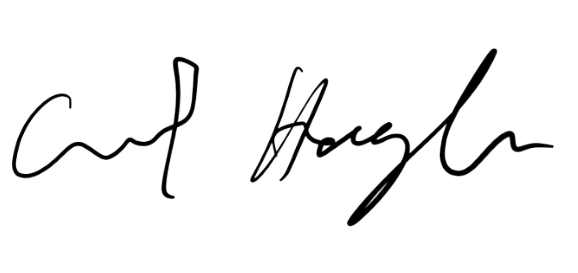
\includegraphics[width=0.2\linewidth]{Conal}\\
		\vspace*{-1.2cm}
		$\ldots\ldots\ldots\ldots\ldots\ldots\ldots\ldots\ldots\ldots$
		\ \\
		Gerard McIntyre - 20332566\\
		\ \\	
		\vspace*{-0.5cm}
		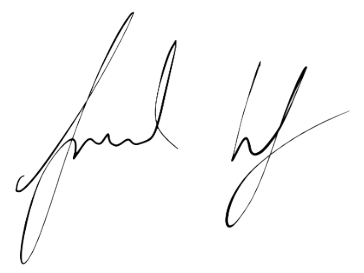
\includegraphics[width=0.2\linewidth]{Gerard}\\
		\vspace*{-2cm}
		$\ldots\ldots\ldots\ldots\ldots\ldots\ldots\ldots\ldots\ldots$
		\ \\
		\vspace*{1cm}
		Amy O'Mara - 20386631\\
		\ \\
		\vspace*{-1cm}
		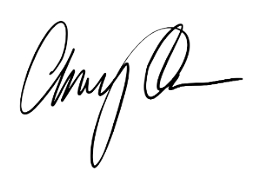
\includegraphics[width=0.2\linewidth]{Amy}\\
		\vspace*{-2cm}
		$\ldots\ldots\ldots\ldots\ldots\ldots\ldots\ldots\ldots\ldots$
		\ \\
		\vspace*{0.8cm}
		Sage Redmond - 20327943 \\
		\ \\		
		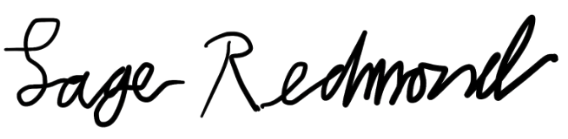
\includegraphics[width=0.2\linewidth]{Sage}\\
		\vspace*{-1cm}
		$\ldots\ldots\ldots\ldots\ldots\ldots\ldots\ldots\ldots\ldots$
		\ \\
		Connall Sharkey - 20389076\\
		\ \\		
		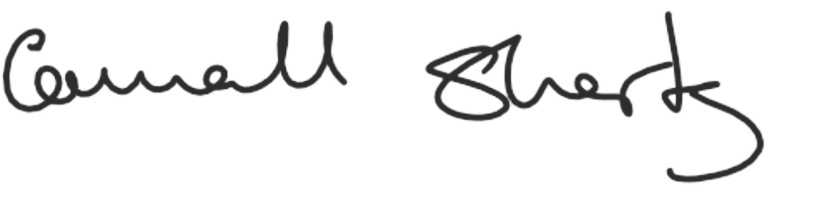
\includegraphics[width=0.25\linewidth]{Sharkey}\\
		\vspace*{-1cm}
		$\ldots\ldots\ldots\ldots\ldots\ldots\ldots\ldots\ldots\ldots$
		\ \\
	\end{flushright}
	\newpage
	
\Large
\section{ACKNOWLEDGEMENTS}
\vspace{-5mm}
\rule{\linewidth}{0.1mm}
\vspace{5mm}\\
\normalsize
Before we start into the heart of the report, we, the authors, would like to formally acknowledge the great assistance that some individuals gave to our group. Firstly, we would like to thank Dr. Bob Lawlor, our lecturer, and co-ordinator, for all the time and effort he gave to further educate us about signals and systems. As well as giving us some of his personal time, to point us in the right direction regarding our project.
\newpage

\Large
\section{INTRODUCTION}
\vspace{-5mm}
\rule{\linewidth}{0.1mm}
\large
\subsection{ASSESSMENT REQUIREMENTS}
\normalsize
The group project must:
\begin{itemize}
	\item Involve a detailed analysis of some variety of information bearing signal.
	\item Involve a frequency-domain analysis of the above signal.
	\item Include at least one convolution operation in both time and frequency domains.
	\item Contain a detailed explanation of the fundamental theory involved.
\end{itemize}
\subsection{OVERVIEW OF CONVOLUTION \& FILTERING}
A filter is a tool or method used in signal processing to eliminate some undesirable elements or characteristics from a signal. 
The whole or part suppression of some characteristic of the signal is what distinguishes filters as a form of signal processing. 
In order to diminish and level out high-frequency noise that is connected to a measurement of flow, pressure, level, or temperature, a signal must first be filtered. 
A mathematical technique called convolution can combine two impulses to create a third signal.
Convolution is therefore crucial in signals and systems since it links the input signal with the system's impulse response to create the output signal.
In other words, the convolution is utilised to represent the relationship between an LTI system's input and output.
\newpage
\subsection{PROJECT OVERVIEW}
The aim of this project was to analyse an information-bearing signal in both time and frequency domains, and to perform some sort of convolution in both domains. The use of theories and practicalities from other modules was heavily encouraged. For this particular project, it was decided to implement a note detector, progressing onto a chord detector. The fundamental idea was to play a guitar chord, process it, isolate the individual notes being played and to output the chord played converted into a piano chord. The microphone input would be using the user’s laptop or computer audio input, and the output would be a UI using a local host.\\
This idea stemmed from the group’s love of music and playing instruments, and we were always fascinated by music technologies such as equalisers. As we had a good knowledge of many programming languages that could be used for a project like this, we decided to implement our own software-based music technology. The language chosen was JavaScript as it seemed to have the most relevant frameworks and libraries, and a UI could be very easily created.\\
Applying our knowledge of Signals and Systems, we formulated the best solution idea we could think of. If we could apply a Fourier transform to a live input in real time, we could isolate the predominant frequencies by filtering out the irrelevant frequencies. This would be done by implementing a band pass filter, setting the lower limit to be the frequency of an open E string and the upper limit to be the highest realistic note on the high E string. A comb filter would then be applied to each note, allowing less than a quarter step either side of the desired note. This could present us with a strange problem in that the comb filter bands are not going to be equal as frequencies increase at an exponential rate.\\
In terms of time domain analysis and convolution, we decided to output the predicted chord onto a keyboard UI and simultaneously play the chord. To play the chord, we would need to incorporate signal synthesising as three or four different notes would be playing, and it would be difficult to get the sound right if all the notes played individually.\\
As multiple people would be working on the same codebase, we decided to set up a GitHub repository (\url{https://github.com/stephengall/EE301_Group_Project}), incorporating some course material from EE308. We realised very quickly we would need to allow for differing ADCs, so some theory from EE302 would also need to be applied. Fourier analysis has been previously taught in EE206, and signal analysis, noise reduction and signal synthesising were all taught in EE213.\\
\newpage

\Large
\section{TECHNICAL BACKGROUND}
\vspace{-5mm}
\rule{\linewidth}{0.1mm}
\large
		\subsection{FOURIER ANALYSIS}
			\normalsize
				\textbf{Fourier Series}

			A Fourier series is a very important area of mathematics developed by Joseph Fourier. It is the representation of a function $f(x)$ in an infinite sum of sines and cosines.
			This can be applied to any function $f(x)$ or any signal, meaning any signal in the universe can be reduced to a sum of sines and cosines. It is used a lot in Signal analysis as it can very easily
			isolate certain frequencies or modify sound waves. The series itself can be expressed in very simple terms. It is comprised of an initial value and an infinite sum of sines and cosines,
			with calculated coefficients. The Fourier series is represented by the following equation:\cite{equation}
$$
				f(x) = \frac{1}{2} a_0 + \sum^{\infty}_{n=1} a_n cos(nx) + \sum^{\infty}_{n=1} b_n sin(nx)
$$
			$a_0$, $a_n$ and $b_n$ can all be calculated as follows:

\begin{align*}
    a_0 &= \frac{1}{\pi} \int^{\pi}_{-\pi} f(x) dx\\
    a_n &= \frac{1}{\pi} \int^{\pi}_{-\pi} f(x)cos(nx) dx\\
    b_n &= \frac{1}{\pi} \int^{\pi}_{-\pi} f(x)sin(nx) dx
\end{align*}

However, for most periodic functions $(f(x) = f(x+2\pi))$ all three values do not need to be calculated. For example, an even function defined as a function $f(x)$ where $f(-x) = f(x)$ will
not need $b_n$ calculated as we know it will be 0. An even function like $cos(x)$ will have no 
sine element to it.

However, for a function that is not symmetric, all three values will need to be evaluated.  
The Fourier series has a very wide range of applications, including signal and spectral analysis, estimating discontinuous functions and convolution \cite{FourierSeries}. However, Fourier series are only the beginning of the wide range of maths that all stem from Joseph Fourier’s discoveries. Fourier series introduce the possibility of the Fourier Transform. The Fourier transform is an extremely powerful tool used in many areas of maths, physics and engineering. It uses different methods of applying the same logic to both continuous and discrete functions and signals.\\ 
\newpage
\vspace*{5mm}
\textbf{Fourier transform and inverse fourier transform}\\
The Fourier transform converts signals and functions from the time domain to the frequency domain, which is central to any system that uses any sort of AC-DC, DC-AC or DC-DC conversion. On top of this, it is used a lot in music as equalisers need to be able to increase or decrease specific frequencies. This is the logic that will be applied for our practical solution. An ADC is used to convert an analogue signal from the time domain to the frequency domain, and then the desired frequencies can be very easily filtered, eliminated or amplified depending on what the system requires.
Again, for such a powerful branch of mathematics, it is a relatively simple equation. For any function $g(t)$, the same equation is applied.

\begin{align*}
    \mathcal{F}\{g(t)\} = G(f) &= \int^{\infty}_{-\infty}g(t) e^{-j2\pi ft}dt\\
    \mathcal{F}^{-1}\{G(f)\} = g(t) &= \int^{\infty}_{-\infty}G(f) e^{j2\pi ft}dt
\end{align*}

Both forms are equally transformable, meaning it is very easy to go from time domain to frequency domain and then back to time domain. While the regular Fourier transform converts from time domain to frequency domain, the inverse Fourier transform converts the other way. This makes DC-AC conversion possible.
\bigskip\\
\textbf{Discrete-Time Fourier Series (DTFS)}\\
Discrete-Time Fourier Series, also known as DTFS, is like the Continuous Time Fourier Series except DTFS produces a periodic sequence. Note that the DTFS can only be applied to a periodic discrete signal. The DTFS is used to represent periodic discrete-time signals in the frequency domain as a weighted combination of complex exponentials.
Consider the discrete signal $x[n]$ = $x[n + N]$, with N being the fundamental period of the signal. The DTFS representation of $x[n]$ can be given by:
$$
    X[k] = \frac{1}{N} \sum^{N-1}_{n=0} x[n]e^{-jk\Omega_0n},k = 0,1,\ldots, N-1
$$
$\omega_0$ = $\frac{2\pi}{N}$, in this case, is the fundamental frequency. Now, given $X[k]$,or the signal in the frequency domain, we can synthesise $x[n]$ using the following equation:
$$
    x[n] = \sum^{N-1}_{k=0} X[k]e^{jn\Omega_0k}
$$
\newpage
If given a continuous signal $x(t)$, $x[n]$ can be found by sampling the signal as seen below.
\begin{figure}[H]
	\begin{center}
		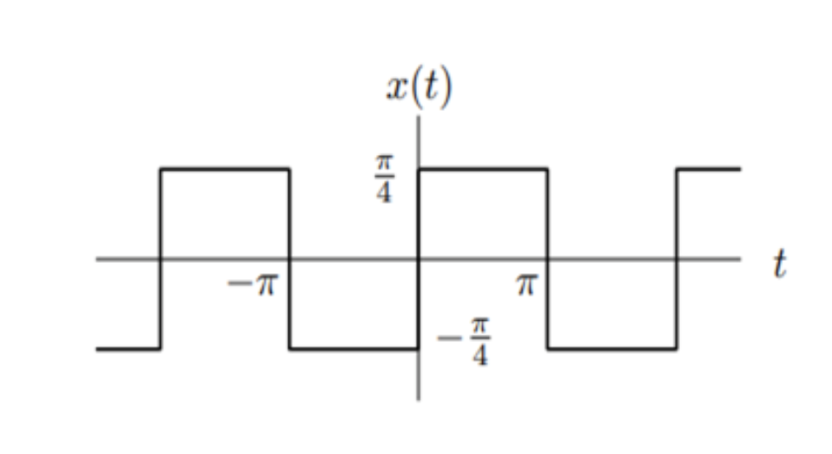
\includegraphics[width=0.6\linewidth]{sampling_1}
		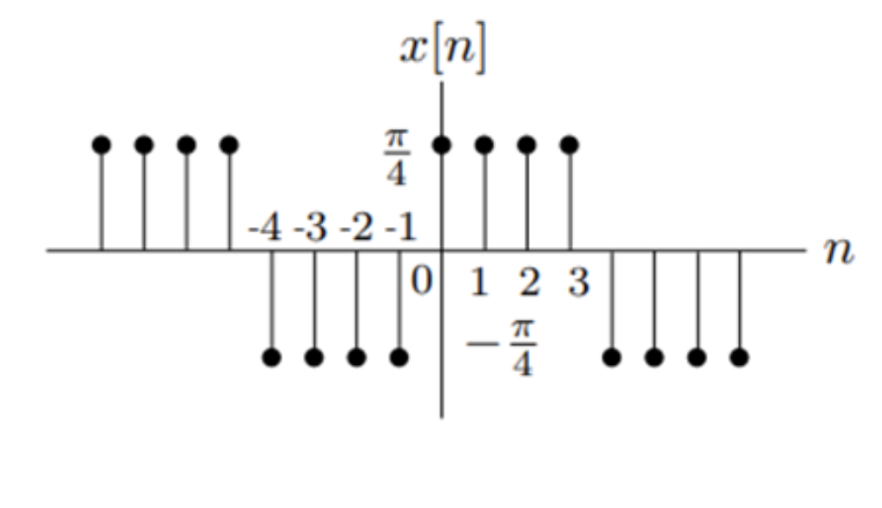
\includegraphics[width=0.6\linewidth]{sampling_2}
	\end{center}
	\caption{Discrete Sampling}
\end{figure}
\bigskip
\textbf{Discrete Fourier Transform (DFT) and Inverse Discrete Fourier Transform (IDFT)}\\
The Discrete Fourier Transform can be applied to discrete periodic time domain signals to represent them in the frequency domain. It is like a normal Fourier transform but instead the integral is replaced by summation and $x(t)$ is replaced by sampled values $x[n]$. It is used to calculate the finite sum of a discrete sequence.
The DFT equation of a signal $s[n]$, is given by:
$$
    S(k) = \sum^{N-1}_{n=0} s[n]e^{-j(\frac{2\pi}{N})kn}
$$
To convert from the frequency domain back to the original time domain signal, the IDFT is applied.
The IDFT is given by:
$$
    s[n] = \frac{1}{N}\sum^{N-1}_{k=0} S(k)e^{j(\frac{2\pi}{N})kn}
$$
In practice, for clarity, $n$ represents the time index and $k$ represents the frequency index.
\newpage
\vspace*{5mm}
\textbf{Discrete-time Fourier Transform (DTFT) and Inverse Discrete-time Fourier Transform (IDTFT)}\\
DTFT applies to discrete aperiodic signals. DTFT is like Fourier Transform (FT) for continuous signals, except the integral is replaced by summation. Also, $x(t)$ is replaced by sampled values $x[n]$. DFT and DTFT are closely related but not identical. DFT provides only non-zero values of one DTFT cycle.
DTFT of a sampled continuous time function $x[n]$ is given by,
$$
	S(k) = \sum^{N-1}_{n=0} s[n]e^{-j(\frac{2\pi}{N})kn}
$$
Inverse DTFT is given by\\
$$
    x[n] = \frac{1}{2\pi} \int^\pi_{-\pi} X(\omega)e^{j\omega n}d\omega
$$
Note that $X(\omega)$ is continuous and periodic (with a period of $2\pi$, i.e.,$X(\omega) = X(\omega + 2\pi)$).\\
\bigskip\\
\textbf{Fast fourier transform (FFT)}\\
Because it works with a limited amount of data, the DFT can be implemented in computers with dedicated hardware or numerical algorithms. The terms DFT and FFT are frequently used interchangeably since DFTs frequently use FFT.
An FFT transform quickly computes the DFT by factorising the DFT and calculating the Fourier Transforms at the same time using matrix operations. This method reduces the big O complexity of the DFT from $O(N^2)$ to $O(Nlog_2(N))$. This significantly shortens the time it takes to compute the DFT, especially when N is set to very large values.
\newpage
\vspace*{5mm}
\begin{figure}[h]
\begin{center}
	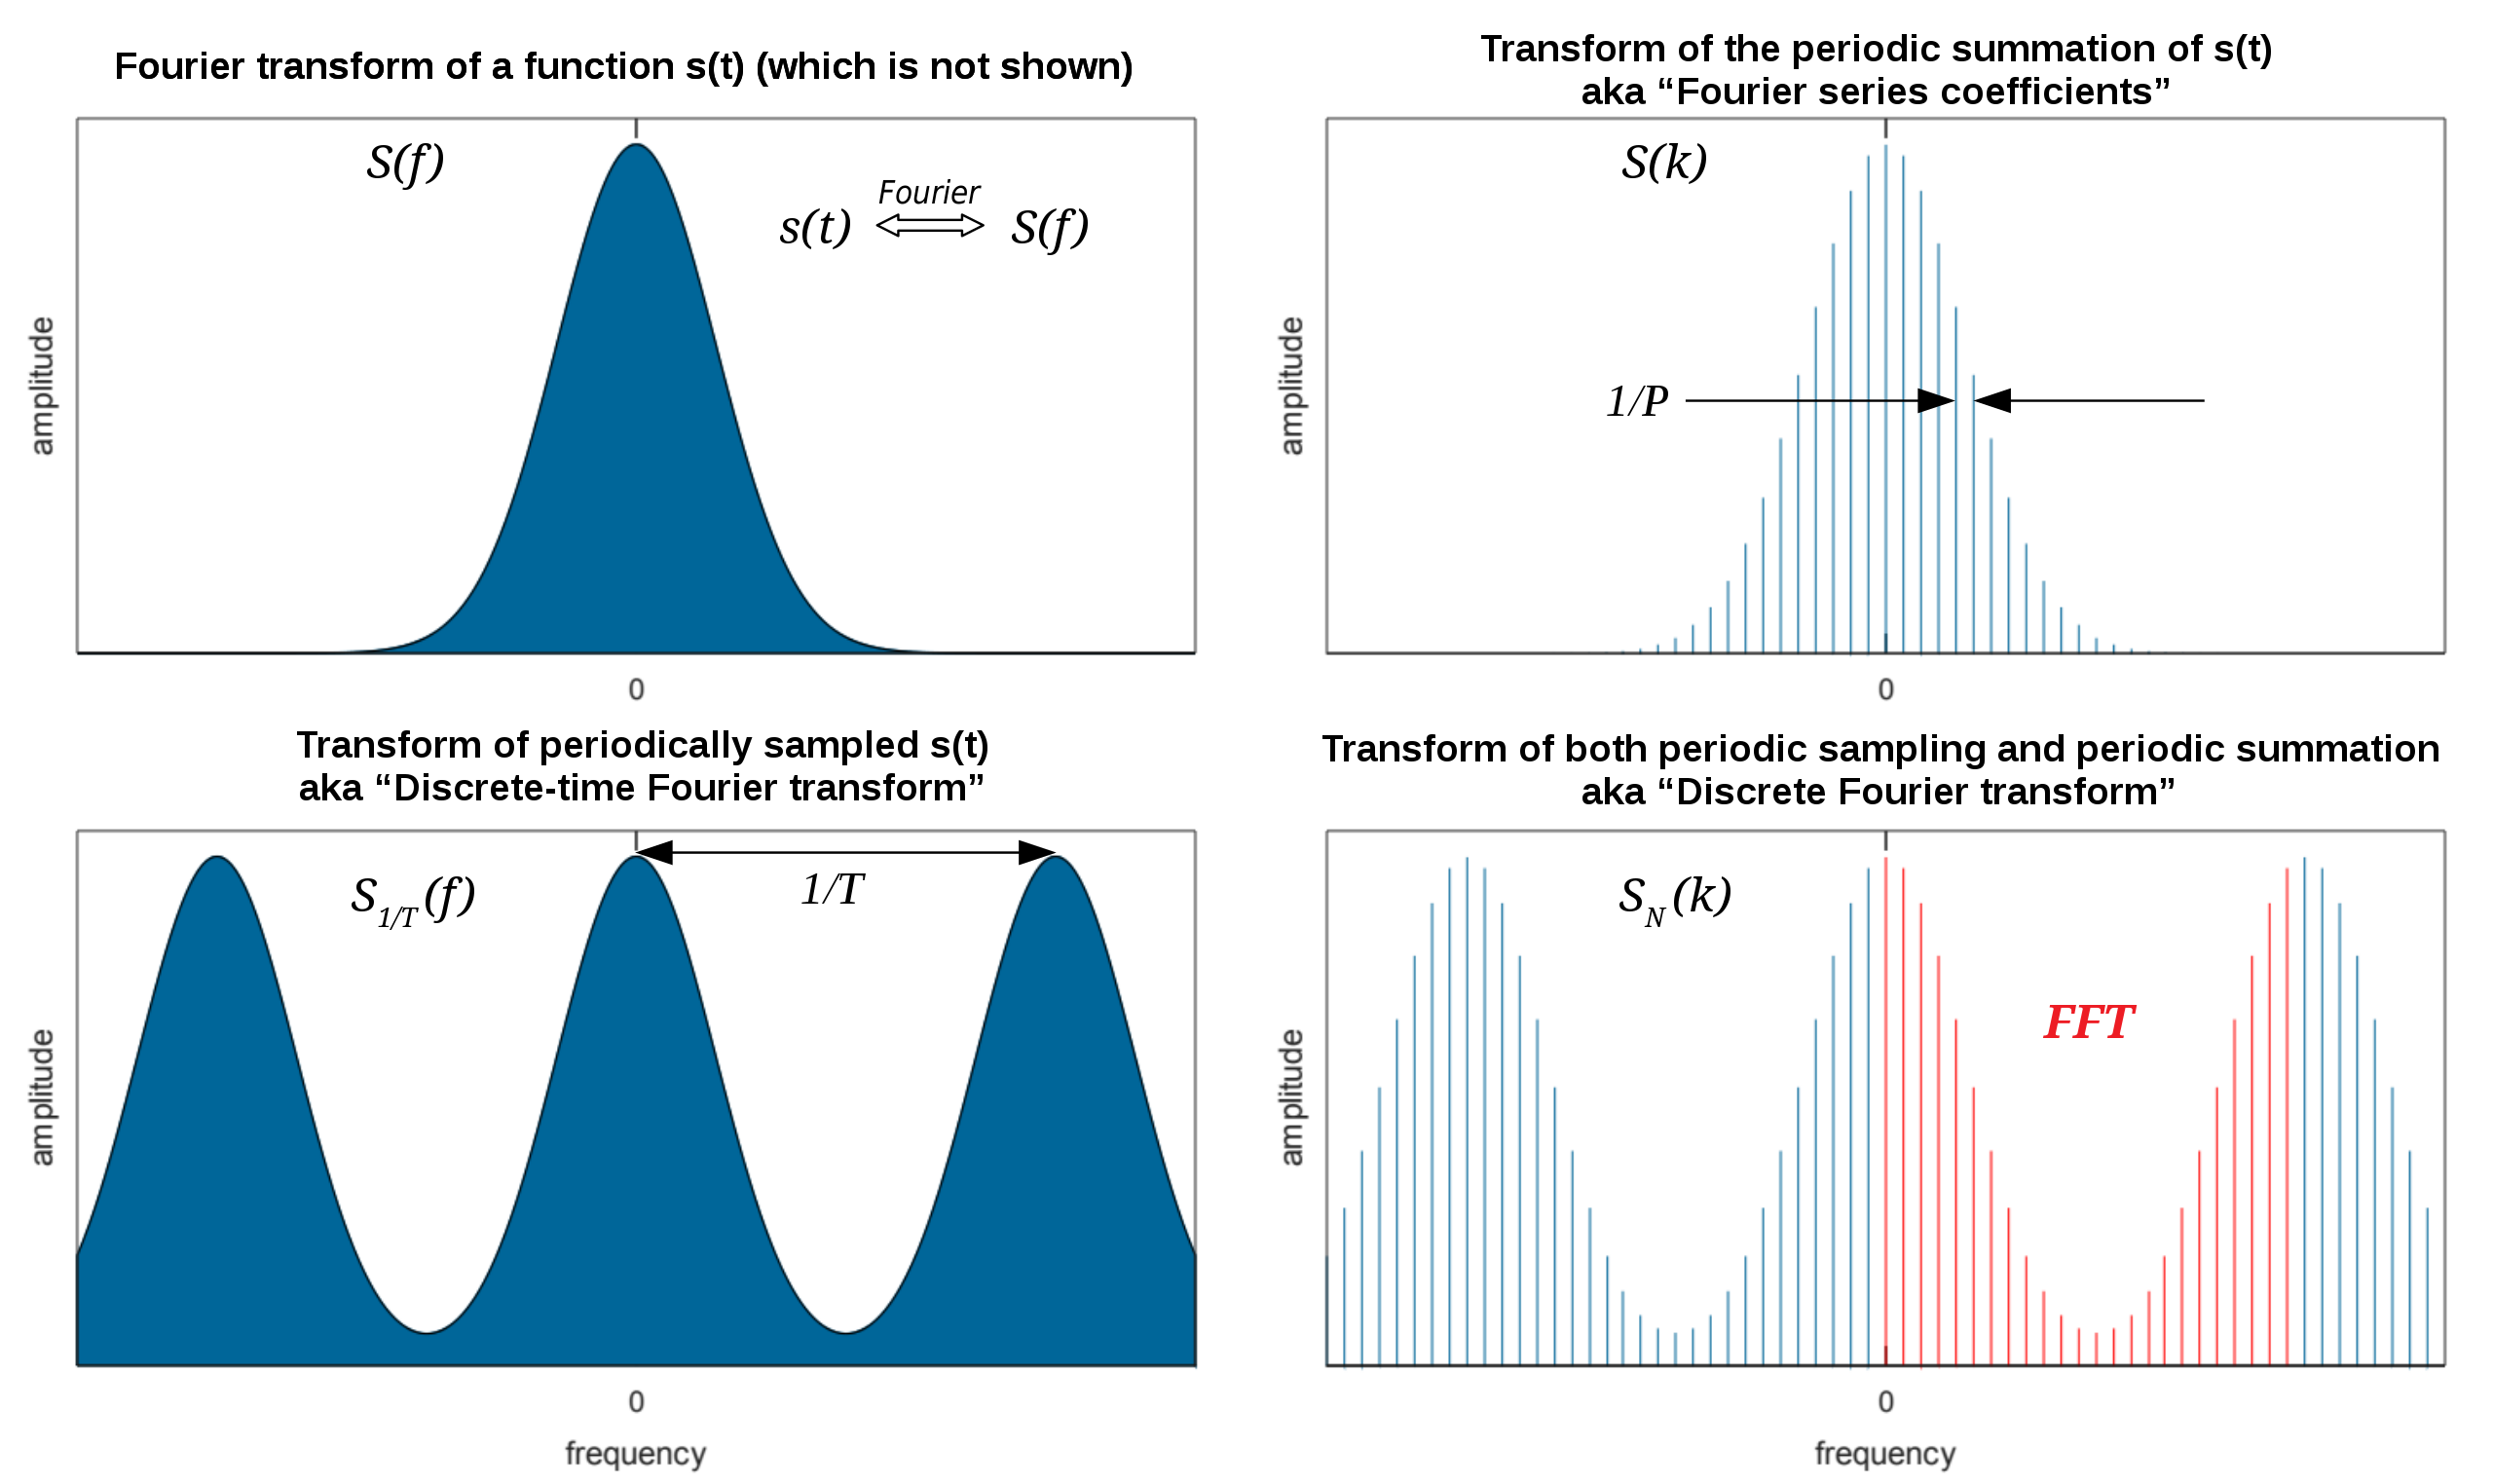
\includegraphics[width=0.7\linewidth]{FFT}
\end{center}
		\caption{Fast Fourier Transform}
		\label{fig:FFT}
\end{figure}
Figure \ref{fig:FFT} is a demonstration of what the differences are between FT, DFT, DTFT. The top left graph is FT, bottom left is DTFT, and lastly bottom right is DFT. Comparing the graphs, it is clear that the DTFT is performing Fourier transform on periodically sampled signals and DFT is showing the summation of sampled points.
\newpage
	\large
	\subsection{MUSIC THEORY}
	\label{sub:MUSIC THEORY}
	
	\normalsize
	Apart from convolution and filtering, this project focuses on the relationship between fundamental music theory and
	frequency. This section covers some important constructs within music theory. Such constructs include chords, pitch,
	notes, root notes, tones and timbre. Each of these are interesting not just from a music theory standpoint, but also
	from a frequency analysis standpoint. \\
	A chord is a combination of two or more notes that are simultaneously played, usually on a musical intrument. This 
	allows a wide range of chords to be created from just twelve notes. Each chord type follows a basic construction. For
	example a major chord is made up of the $1^{st}$, $3^{rd}$ and $5^{th}$ notes of the major scale. \\
	The simplest major chord as a C major, as its scale contains no sharps or flats. The scale is given by:
	C,D,E,F,G,A,B. Therefore the major chord can be given by C, E and G. The root note is the base of this chord, C.\\
\begin{figure}[h]
\begin{center}
		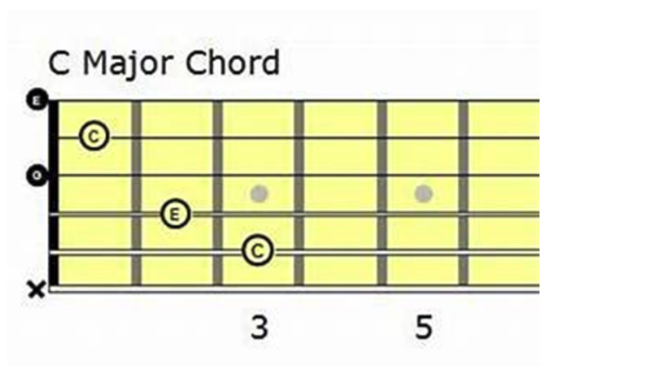
\includegraphics[width=0.7\linewidth]{C_chord}
	\end{center}
	\caption{C major as played on guitar}
\end{figure}
\newpage
\vspace*{5mm}
	A note is produced by certain frequencies made by vibrations. These vibrations can be made by strumming a string or even by changing the level of air exhaled from  lungs that pass through the vocal cords.
	If the frequency is higher, a higher pitch note is produced. If an $A_{4}$ ($440Hz$) and $A_{3}$ ($220Hz$) are played, the 
	$A_{4}$ is at a higher pitch. The number after the note signifies at which octave the note is being played. "Middle C" on
	a standard 88 key piano is $C_{4}$, as it is the $4^{th}$ C note on the instrument.\\
	The relationship between a change in note and a change in frequency is shown with the following equation:
	$$
		halfToneHigher(Hz) = note * 2^{\frac{1}{12}}
	$$
	Where the $\frac{1}{12}$ gives the change in note. One half tone is $\frac{1}{12}$, a full tone is $\frac{2}{12}$, etc.
	For example if the frequency of C\# is desired and C natural is given as $262Hz$, C\# can be found as follows:
	$$
		C\# = 262 * 2^{\frac{1}{12}} \Longrightarrow 277.58Hz
	$$

	Knowing this, another musical idea can be introducedto compare notes, namely tones. 
	Most would agree that the term 'tone' can just be used hand in hand with note, while others would argue that a tone is a single pitch, and a note is a pitch with overtones. 
	It is widely accepted that it is the former. 
	Tones are more so associated with another new term, a 'step'.
	A half-tone is a half-step and a whole-tone is a whole-step etc. 
	A half-step, for example, is a C to a C\#.
	A whole step would be from a C note to a D note.
	A tone or note can be described by its pitch, duration and volume.
\newpage
\vspace*{5mm}
\begin{figure}[h]
	\begin{center}
		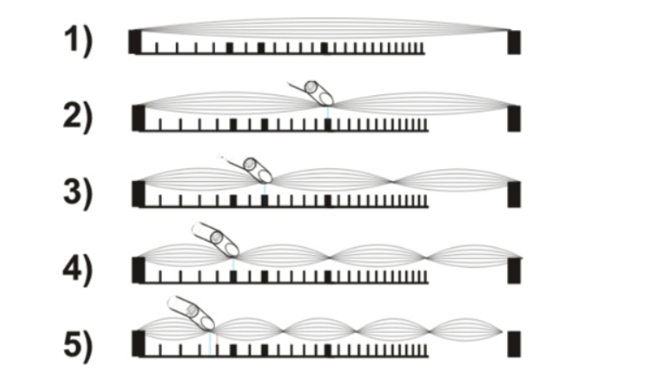
\includegraphics[width=0.7\linewidth]{Harmonics}
	\end{center}
	\caption{Harmonics}
	\label{fig:HARMONICS}	
\end{figure}
	Figure \ref{fig:HARMONICS} demonstrates how the placement of the finger on a string controls the vibration of the string, hence controlling the notes produced when the string is plucked. The numbers $1-5$ represent the first five 
	harmonics. A harmonic is a multiple of the fundamental frequency. The fundamental frequency begin the lowest
	resonant frequency of a vibrating object.\\
	One more phenomenon that influences how a piece of music sounds is timbre. Timbre is what makes the same piece
	of music played on two different instruments sound completely different. Comparing instruments from various families brings out the effect of timbre the most; for example, brass instruments have a drastically distinct timbre from string instruments. 
	Timbre can be assessed by recalling the fundamental frequency of an instrument.
	It is known that lower-frequency instruments produce more audible harmonics or overtones than high-frequency ones. In other terms, certain types of instruments focus on producing the fundamental frequencies, while others focus on overtones.\\
	Music, notes and sound in general can be seen as an addition of multiple sine waves. 
	The Fourier series can be used to represent any periodic sound. In fact, strings and tubes can be used to mimic the sounds of numerous instruments by combining a variety of harmonics to create a fundamental timbre.
	This process is known as additive synthesis.
\newpage
\vspace*{5mm}
\begin{figure}[H]
\begin{center}
		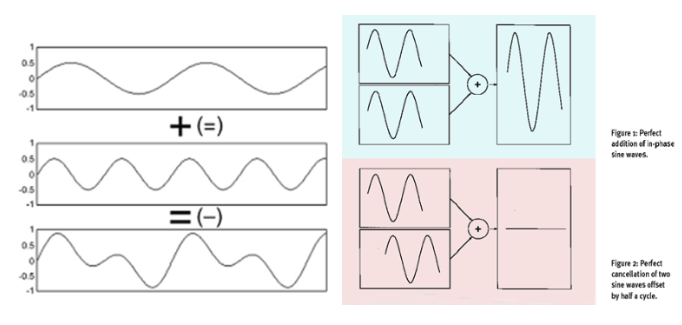
\includegraphics[width=0.7\linewidth]{synthesis}
	\end{center}
	\caption{Additive Synthesis}
\end{figure}
	The summation of multiple waves can produce much more complicated waveforms. 
	The addition of two waveforms of equal amplitude and phase produces an amplification affect, while two waveforms
	out of phase can negate each other.
\newpage
	\subsection{CONVOLUTION}
		\normalsize
		When two signals combine, the output waveform will be the convolution of the previous two signals. Convolution is a mathematical function. The characteristic and structure of either of the first
		two signals will have an impression on this convoluted signal. The equation below highlights the continuous time operation, where $x(t)$ and $h(t)$ are the two signals that must be convolved, where 
		$y(t)$ is the new convoluted signal,  where $\tau$ is a variable of integration, and $t$ is absolute time.
				$$
					y(t) = x(t)\cdot h(t) = \int_{-\infty}^{\infty} x(\tau) h(t - \tau)d\tau 
				$$
		The equation below highlights the discrete time operation, where $x[n]$ and $h[n]$ are the two signals that must be convolved, where $y[t]$ is the new convoluted signal and where $n$ and $k$ are
		index variables.
				$$
					y[n] = x[k]\cdot h[k] = \sum_{k=-\infty}^{\infty}x[k]h[n - k]
				$$
		A three-cycle sine wave and a gradually increasing ramp are used as the input signals in an example of low-pass and high-pass filtering using convolution. In the low-pass filter(Figure \ref{fig:LOWPASS})\cite{LowPass}, the impulse response is a ramp pulse that is sent to the output because the impulse response is a seamless arch. Similar to Figure \ref{fig:HIGHPASS}, only the sinusoid that oscillates more quickly is allowed to pass.
	\begin{figure}[H]	
		\begin{center}
			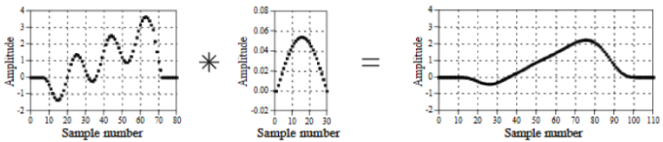
\includegraphics[width=0.7\linewidth]{Lowpass_sig}
			\caption{Lowpass Filtering Example}
			\label{fig:LOWPASS}
			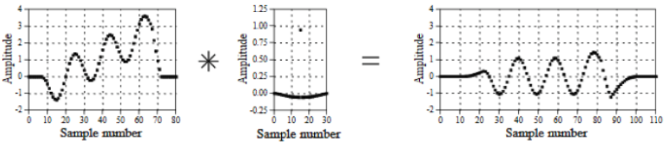
\includegraphics[width=0.7\linewidth]{Highpass_sig}
			\caption{Highpass Filtering Example}
			\label{fig:HIGHPASS}
		\end{center}
	\end{figure}
		The practice of using convolution has very useful applications such as probability, statistics, acoustics, spectroscopy, signal processing and image processing, geophysics, engineering, physics, computer vision and neural networks.
		\large
\newpage
	\subsection{FILTERING}
		\normalsize
		Filters are used to process signals by allowing certain frequencies to pass through while blocking or attenuating other frequencies. They can be used to eliminate unwanted noise, reduce
		interference, or shape a signal. Signal filters are commonly described in terms of frequency response, which is the measure of how a filter responds to different frequencies. This is often
		expressed as a frequency response function, which describes the gain or attenuation of a signal at different frequencies. Signal filters can be implemented in either the analogue or digital domain
		and can be either active or passive components.
		The following are ideal filters. Ideal filters are not realistically feasible but rather serve as a mathematical idealisation of practical filters.

		
			\subsubsection{Analogue Filtering}
				The design of analogue filters is based on a combination of inductors, capacitors, and resistors, which are arranged in a specific configuration to allow or reject certain frequencies.
				Analogue filter design includes transfer functions, poles and zeros, frequency response, output response, all of analogue filters\cite{AnalogueFilters}. The filter's behaviour is determined by the magnitude and phase of its frequency response, which is determined by the filter's transfer function. These filters
				approximate frequency response of ideal filters by a rational transfer function\cite{EE213}. Analogue filters are more subjected to non-linearity
				and often results in smaller accuracy because they rely on electrical components that may have inherent inaccuracies and can be subject to outside disturbances\cite{SignalSuppression}. Although a benefit of using these is that they have greater high frequency filtering,
				low latency and speed, which can be up to 100 times as fast, as opposed to digital filters.\\
\newpage
\vspace*{5mm}
\textbf{Lowpass Filtering}\\
				A lowpass filter is a type of electronic filter that passes low-frequency signals but attenuates (reduces the amplitude of) signals with frequencies higher than the cutoff frequency. 
				The lowpass filter is based on the principle of frequency-selective attenuation, whereby signals with frequencies within a certain range are allowed to pass while frequencies outside
				of this range are attenuated. Lowpass filters can be used in many different applications such as audio, video, and telecommunications.
					
				\begin{figure}[H]
					\begin{center}
						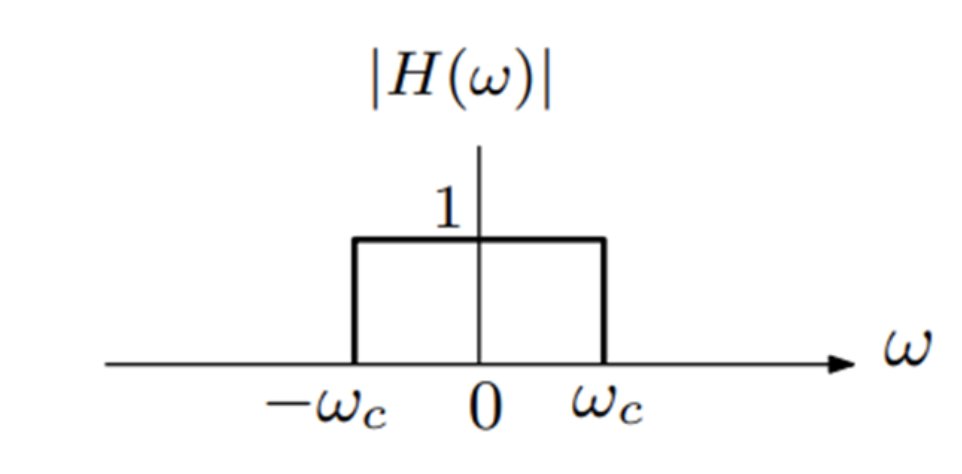
\includegraphics[width=0.6\linewidth]{Lowpass}
							\caption{Active Lowpass Response}
						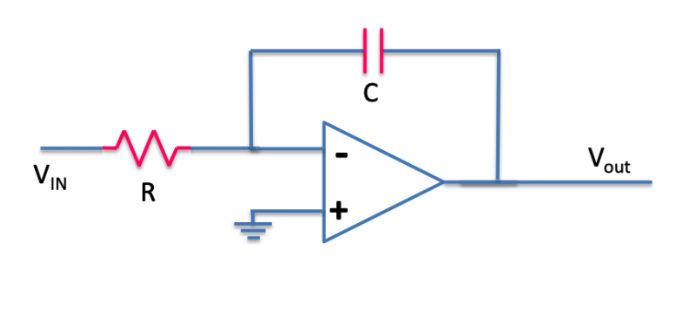
\includegraphics[width=0.6\linewidth]{Lowpass_circuit}
							\caption{Active Lowpass Circuit}
							\label{fig:LOWPASS_CIRCUIT}
					\end{center}
				\end{figure}
By connecting a single resistor and a single capacitor in series as shown in Figure \ref{fig:LOWPASS_CIRCUIT}, it is simple to manufacture a low pass filter. The input signal (VIN) is applied to the series combination (both the resistor and the capacitor together) in this type of filter design, but the output signal (VOUT) is taken just across the capacitor.				
\newpage
\vspace*{5mm}
			\textbf{Highpass Filtering}\\
				A highpass filter is a type of frequency-dependent filter that passes frequencies above its cutoff frequency, while attenuating frequencies below the cutoff. This is accomplished
				by allowing the high frequency signals to pass through the filter with minimal distortion while blocking the low frequency signals. The cutoff frequency is determined by the filter's
				design and is typically set to a frequency that is slightly above the desired signal's frequency range.
				\begin{figure}[H]
					\begin{center}
						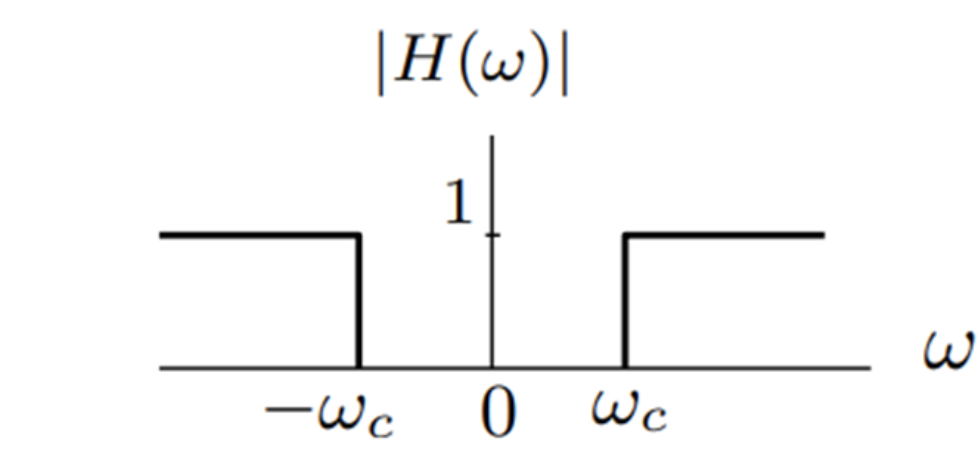
\includegraphics[width=0.6\linewidth]{Highpass}
						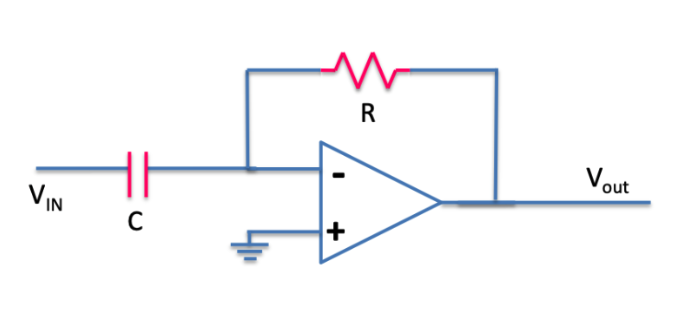
\includegraphics[width=0.6\linewidth]{Highpass_circuit}
					\end{center}
					\caption{Active Highpass Response and Circuit}
				\end{figure}
			\textbf{Bandpass Filtering}\\
				A bandpass filter is an electronic filter designed to allow signals within a certain frequency band to pass, while rejecting signals outside of that band. It typically consists of a
				series of inductors and capacitors connected in a circuit to form a resonant circuit; this is known as a passive bandpass filter. Other filters require an external source of power and
				employ active components such as transistors and integrated circuits; these are known as active bandpass filters.\cite{Bandpass}
				When a signal is applied, the filter passes the frequencies within the designated band, while attenuating or blocking frequencies outside of the band.
				\begin{figure}[H]
					\begin{center}
						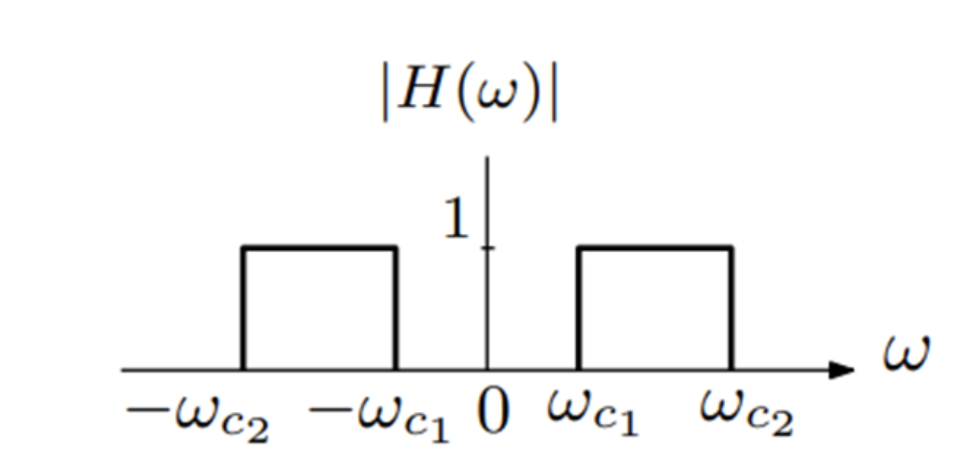
\includegraphics[width=0.6\linewidth]{Bandpass}
						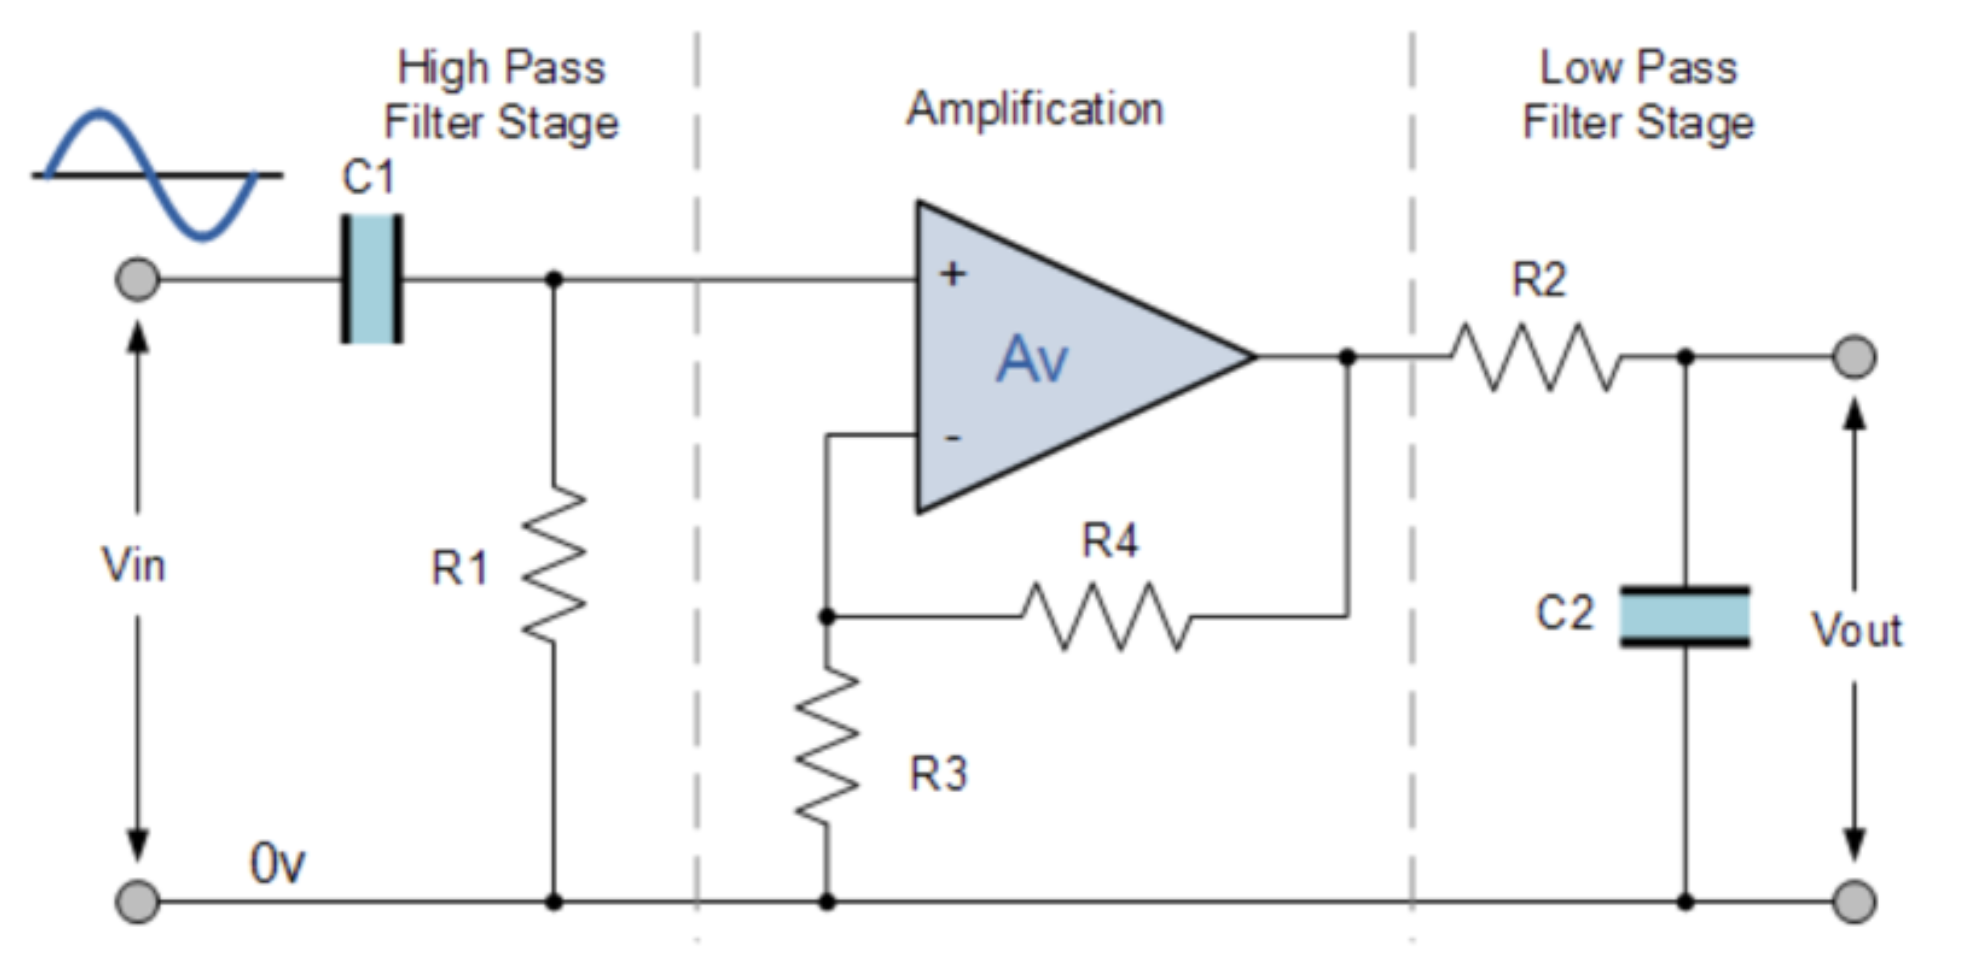
\includegraphics[width=0.6\linewidth]{Bandpass_Circuit}
					\end{center}
					\caption{Bandpass Response and Circuit}
					\label{fig:BANDPASS}
				\end{figure}
				A Bandpass filter circuit with a broad pass band is created by pooling together the individual low and high pass passive filters. The high pass part, which makes up the first process of the filter, uses the capacitor to prevent any DC biassing from the source. With one half representing the low pass response and the other half representing the high pass response, as depicted in Figure \ref{fig:BANDPASS}, this design has the advantage of creating a generally smooth asymmetrical pass band frequency response.
\newpage
\vspace*{5mm}
			\textbf{Bandstop Filtering}\\
				A bandstop filter is a type of filter that is used to reject a certain range of frequencies from an incoming signal. It works by passing signals of frequencies outside this range,
				while attenuating or filtering out signals of frequencies within the specified range. This type of filter is sometimes referred to as a notch filter because it is designed to create
				a “notch” in the frequency response of the system. Bandstop filters are typically used to reduce interference from undesired frequency bands in a signal, such as radio frequencies.
				\begin{figure}[h]
					\begin{center}
						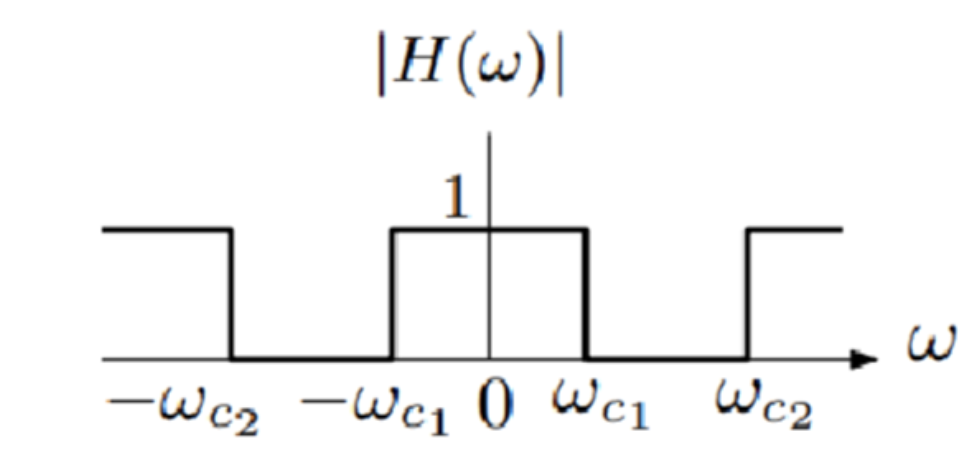
\includegraphics[width=0.6\linewidth]{Bandstop}
						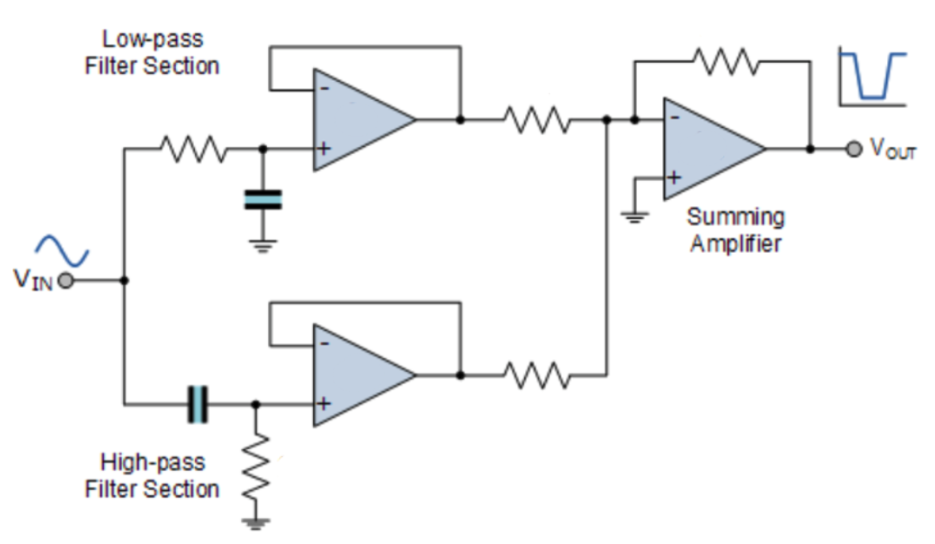
\includegraphics[width=0.6\linewidth]{Bandstop_circuit}
					\end{center}
					\caption{Bandstop Response and Circuit}
				\end{figure}
				Instead of using a cascading connection to merge the low pass and high pass filters, the band stop filter is created using a parallel connection. The properties of a band-stop filter are the exact opposite of those of a band-pass filter. Low frequencies from the original signal are transmitted through the band stop circuit's low pass filter, and high frequencies from the original signal are transmitted through the high pass filter.\\	
\newpage
			\textbf{Butterworth Filtering}\\
				A Butterworth filter is a type of signal processing filter designed to have a frequency response which is maximally flat in the passband. It is also characterized by a steep roll-off 
				rate in the stopband, meaning that the frequency response at the stopband edge is much lower than that at the passband edge.
						The Butterworth filter has a flat frequency response. The amplitude response $|H(\omega)|$ of an Nth-order Butterworth low pass filter is given by:
						$$
    						|H(\omega)| = \frac{1}{\sqrt{1 + (\frac{\omega}{\omega_c})^{2N}}}
						$$
			\begin{figure}[H]	
				\begin{center}
					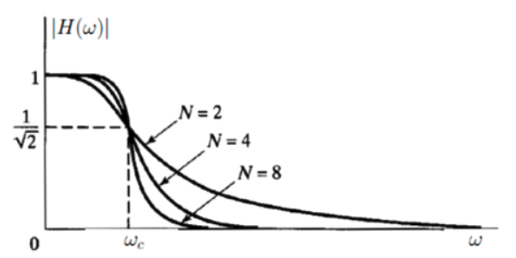
\includegraphics[width=0.7\linewidth]{Butterworth_graph_2}
				\end{center}
				\caption{Butterworth Response}
			\end{figure}
					The gain drops by a factor  at $\omega = \omega_{c}$ for all N. We call $\omega_{c}$ the half-power frequency or $3dB$ cutoff frequency for this reason. We can also observe that the amplitude response decreases
				monotonically with $\omega$ and for large N the amplitude response approaches ideal characteristics\cite{AnalogueFilters}.
				The analogue low pass filter's 'brick wall' can be defined as standard approximations for various filter orders, as shown below\cite{SignalSuppression}.
			\begin{figure}[H]				
				\begin{center}
					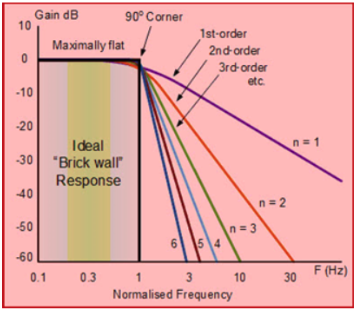
\includegraphics[width=0.7\linewidth]{Butterworth_graph_1}
				\end{center}
				\caption{Butterworth Bode Plot}
			\end{figure}
				If the order increases, then the filter design stages also increase. As such, the filter and the “brick wall” response gets closer.[2] The filter is often used in applications 
				such as audio processing, image processing, and circuit design. Butterworth filters are named after British engineer and physicist Stephen Butterworth who first described
				them in his 1930 paper entitled "On the Theory of Filter Amplifiers".
\newpage
\vspace*{5mm}
			\textbf{Chebyshev Filtering}\\
				Chebyshev filter design is a type of linear filter that is designed to pass a range of frequencies with minimal attenuation, while rejected a range of frequencies with maximal attenuation. Attenuation refers to the reduction in strength or intensity of a signal as it travels through a medium or over a distance. They are characterised by their steep roll-off and sharp transition between the passband and stop band. There are two types: low-pass and high pass.
				\begin{figure}[H]
					\begin{center}
						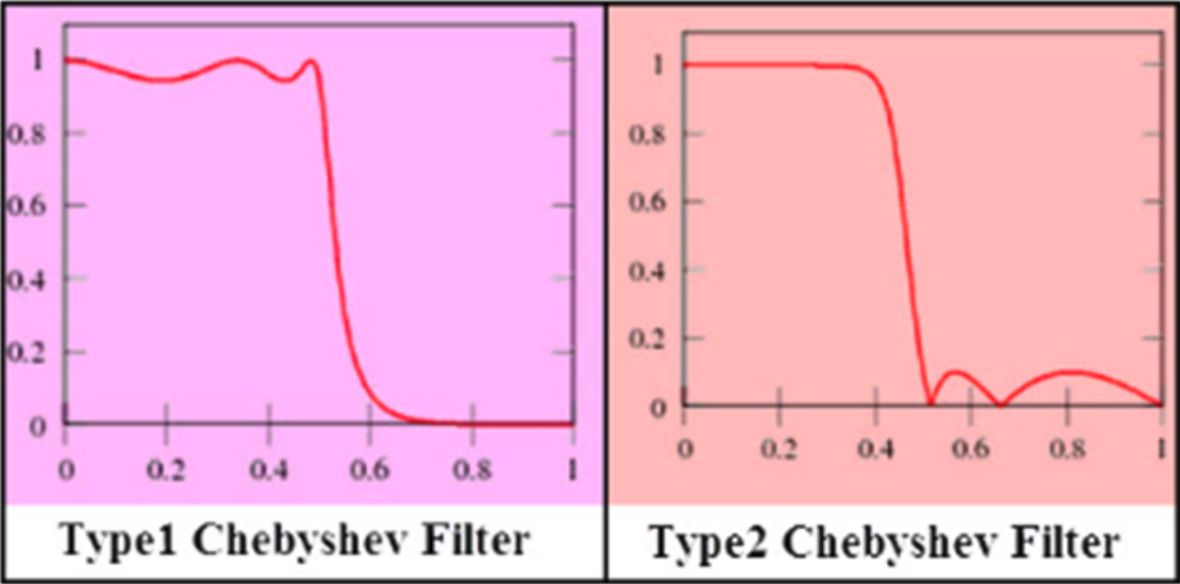
\includegraphics[width=0.7\linewidth]{Chebyshev_response}
					\end{center}
					\caption{Chebyshev response}
				\end{figure}
			Type 1 filters are the most common, the passband exhibits a ripple behaviour and then continues to drop into the stopband as the frequency increases. Type 2 filters are also known as inverse Chebyshev filters, they are less common because it does not roll off as fast as type 1 and requires more components. It has no ripple in the passband but does in the stopband. The order of a Chebyshev filter is equal to the number of reactive components, i.e. inductors\cite{Chebyshev}.
			These filters are commonly used in electronic circuits for filtering out unwanted frequency components from a signal.\\
			\textbf{Active Vs Passive Filtering}\\
			Active and passive filters are two categories into which filters can be subdivided. Active filters are produced from active components like amplifiers in tandem to passive components, whereas passive filters are made from passive components like resistors, capacitors, and inductors. While passive filters do not necessitate a power source to perform, active filters do. Active filters maintain their performance regardless of the connected load, while passive filters' output varies with the load. Active filters can enhance the signal's gain while passive filters cannot. Active filters sustain the signal's amplitude regardless of whether no gain is provided, whereas passive filters reduce the signal's overall strength.
			\newpage
			\subsubsection{Digital Filtering}
			Digital filters are a type of mathematical operation that is applied to a digital signal. These filters can be used to smooth out noise, emphasise features of a signal, and remove unwanted frequencies of the signal. They operate by convolving the input signal with a set of coefficients, also known as weights, to produce an output signal. The weights are chosen based on the desired output and can be adjusted to achieve the right response.
Digital filters are used in many scientific and engineering applications such as control systems, image and signal processing, and communications. They are very important when extracting information from large and complex data sets. These filters can be used in the design of finite impulse response filters, equivalent analogue filters are often more complicated as they require delay elements \cite{Digital_Filtering}.

			\textbf{FIR Filtering}\\
			Finite Impulse Response (FIR) filters are a type of filter used in signal processing. They are linear and time invariant, meaning that their output is determined solely by their input and their internal structure, and their response will remain the same regardless of when they are applied. They work by passing an input signal through a series of weighted delays or taps, where each tap has a coefficient associated with it. When the signal passes through the taps, the coefficients are multiplied with the signal resulting in an output that is a weighted sum of the input signal. FIR filters are used to attenuate or amplify certain frequencies in a signal, or to shape the frequency response of a system.\\
			Characterised by:
			$$
				y[n] = \sum_{k = 0}^{M - 1}h[k]x[n - k]
			$$
			Where $h[0]$, $h[1]$, $\ldots$, $h[M-1]$ are M filter coefficients.\\
			An FIR filter can be obtained by implementing there elements: Addition, multiplication by a constant and delay blocks\cite{FIR}.
			\begin{figure}[H]
				\begin{center}
					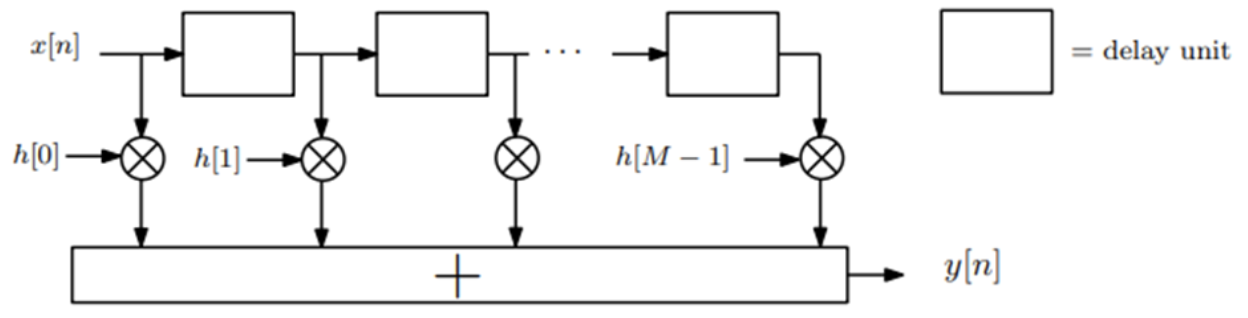
\includegraphics[width=0.7\linewidth]{FIR}
				\end{center}
				\caption{FIR Layout}
			\end{figure}

			\textbf{IIR Filtering}\\
			An IIR filter is a type of digital filter that uses a recursive algorithm to process digital signals and can be used to create a linear system with an infinite response to an impulse. The input signal is combined with a feedback signal from the output of the filter. The output of the filter is then used to generate the feedback signal for the next iteration. This feedback loop allows the filter to have a more complex frequency response than other types of digital filters, such as FIR filters.\\
			\begin{figure}[H]
				\begin{center}
					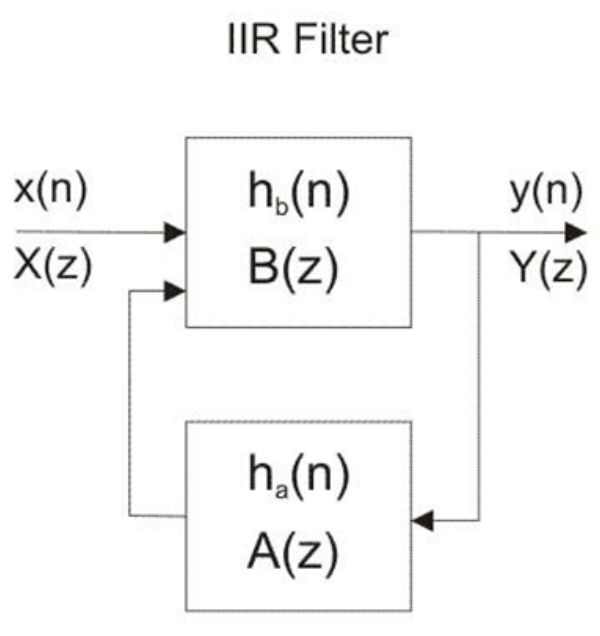
\includegraphics[width=0.5\linewidth]{IIR}
				\end{center}
				\caption{IIR Layout}
			\end{figure}
			The IIR filter is unique because it uses a feedback mechanism. It requires current as well as past output data. Though they are harder to design, IIR filters are computationally efficient and generally cheaper\cite{IIR}.			
			IIR filters are often used for audio processing, noise reduction, and equalisation. They are less computationally intensive and are therefore used in software.\\
			\textbf{ICR Filtering}\\
			An Integrated Circuit Resistor is a type of signal processing used to reduce the number of unwanted components in a signal. It is based on the concept of IIR filtering. The ICR uses an IIR filter to reduce the presence of high-frequency components in a signal. This is done by passing the signal through an IIR filter with a cut-off frequency determined by the user. The ICR filter then uses an inverse filter to invert the high-frequency components and remove them from the signal. This effectively reduces the presence of unwanted high-frequency components in the signal, resulting in a cleaner and more accurate signal.
			\\\textbf{Comb Filtering}\\
			Comb filtering occurs when two or more signals with the same or similar frequencies are combined with a very short delay in between, between 75us to 15ms\cite{COMB_2}. This can occur when multiple microphones are used to capture the same sound source. Steep notches appear in the resulting audio at repeating frequency intervals, similar to that of a comb.
			\begin{figure}[H]
				\begin{center}
					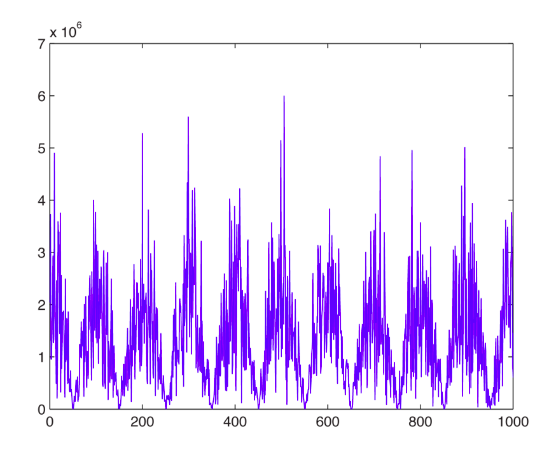
\includegraphics[width=0.5\linewidth]{Comb_Filter}
				\end{center}
				\caption{Comb Filter Layout}
			\end{figure}
			This filtering distorts the original sound and can result in it sounding 'hollow'. This can be avoided in multiple ways such as:\\
			\begin{enumerate}
				\item Implementing a phase shift. A phase shift associated with high pass filters and low pass filters can be very effective in preventing comb filtering.\\
				\item Adjusting the delay by aligning them perfecting can also seamlessly remove a comb filter\\
			\end{enumerate}  
			The resonance or attenuation of the frequencies caused by the delay is dependent on the amount of time it is delayed by\cite{COMB}. If a component is delayed by exactly one cycle or period and mixed with the original sound then it will be reinforced. Also, if it is delayed by a half period then it will be cancelled.
			They can be used to create a variety of interesting effects in audio, such as harmonising. Comb filters can create or enhance harmonics in an audio signal. If the filter has a delay time that is an integer multiple of the fundamental frequency of a harmonic series, then it can be used to boost the harmonics of that series. 

\newpage
			\subsection{CONVERSION}
			AC stands for alternating current, current that changes direction and flows forward and backward. It has non-zero frequency. DC stands for direct current, current that doesn’t change its magnitude or polarity. It has zero frequency.\\
			\textbf{AC-DC}\\
			The process of the conversion of AC current to DC current is known as rectification. There are 4 steps involved in this conversion.\cite{ACDC}\\
			\begin{enumerate}
				\item Stepping down the voltage levels. Often voltage levels are increased when sending power over long distances so a step-up transformer is used. But when a device needs lower power, a step-down transformer is used. The transformer uses a ratio to output the corresponding voltage from what was inputted.
				\item Create an AC to DC power converter circuit using a rectifier. There are different types of rectifiers such as half-wave, full-wave and bridge rectifiers. The input AC power will be rectified into output DC power, but it consists of pulses and is not pure DC.
				\item Obtain the pure DC waveform. This can be done using a capacitor. A capacitor stores energy which the input voltage increases from zero to its peak value. The energy from the capacitor can be discharged while its input voltage is decreasing. The pulsating DC is converted into pure DC using this method.
				\item Regulating fixed DC voltage is done by using a voltage regulator IC. DC voltage regulator ICs are named 78XX with the last two digits representing the output voltage value so you use the IC that fits the desired voltage output.
			\end{enumerate}
			Applications of AC-DC conversion include almost all electronics and electrical devices. They are used as power supply circuits for appliances such as computers, chargers, refrigerators. Most electronics sensors and modules only operate on DC supply so they need the AC to be converted before use.
			\\\textbf{DC-AC}\\
			DC can be converted into AC using an inverter in two steps.\cite{DCAC}
			\begin{enumerate}
				\item Turn DC into AC. In a circuit, a switch can be implemented that alternatively turns on and off the DC straight line signal. To make the current flow in both directions, an inverter uses a 4-way switching bridge of transistors to re-route the direct current to alternate it. To transform it into a wave, diodes may be used to smoothen the signal from a step response to a pure sine wave.
				\item Step-up the voltage. As mentioned above, a step-up transformer increases the voltage levels. It is made up of a primary and secondary coil. The current passes through one coil and to the other using electromagnetic induction. The wiring density is directly related to the increased voltage output.
			\end{enumerate}
			Applications of DC-AC conversion include solar panels, car batteries and wind turbines.
			\\\textbf{DC-DC}\\
			DC to DC converters store energy so it can be converted at one voltage to another. This is applied when, in a large system of varying components, some components may need a much higher voltage than the rest or vice-versa \cite{DCDC}
			These are done using step-up DC-DC and step-down DC-DC converters. The input and output power is always maintained, input voltage x input current = output voltage x output current. Step-up converters are often used in heavy machinery, lighting systems and AM/FM sound systems. Step-down converters would be used for power supplies for electronic devices in industrial control and automotive systems.
			\\\textbf{Clipping}\\
			An AC voltage is used to represent audio when acoustic signals are transformed into electrical signals (using a microphone or instrument pickup). The voltage of this AC signal must be raised to increase the audio output's volume. In order to accomplish this, amplifiers with gain-enhancing hardware are used. The power source has restrictions on the maximum magnitude of the signal that can be transmitted, clipping occurs at these voltage rails. It is impossible to magnify the incoming signal after the maximum power supply voltage has been reached without affecting its shape. This denotes an amplified but severely distorted rendition of the signal. The graphic below shows two sine waves. The bottom sine wave surpasses this restriction, while the top sine wave stays within them. The signal was "clipped," resulting in the flattened blue lines. The sine output signal loses its rounded peaks and troughs \cite{CLIPPING}.
			\begin{figure}[H]
				\begin{center}
					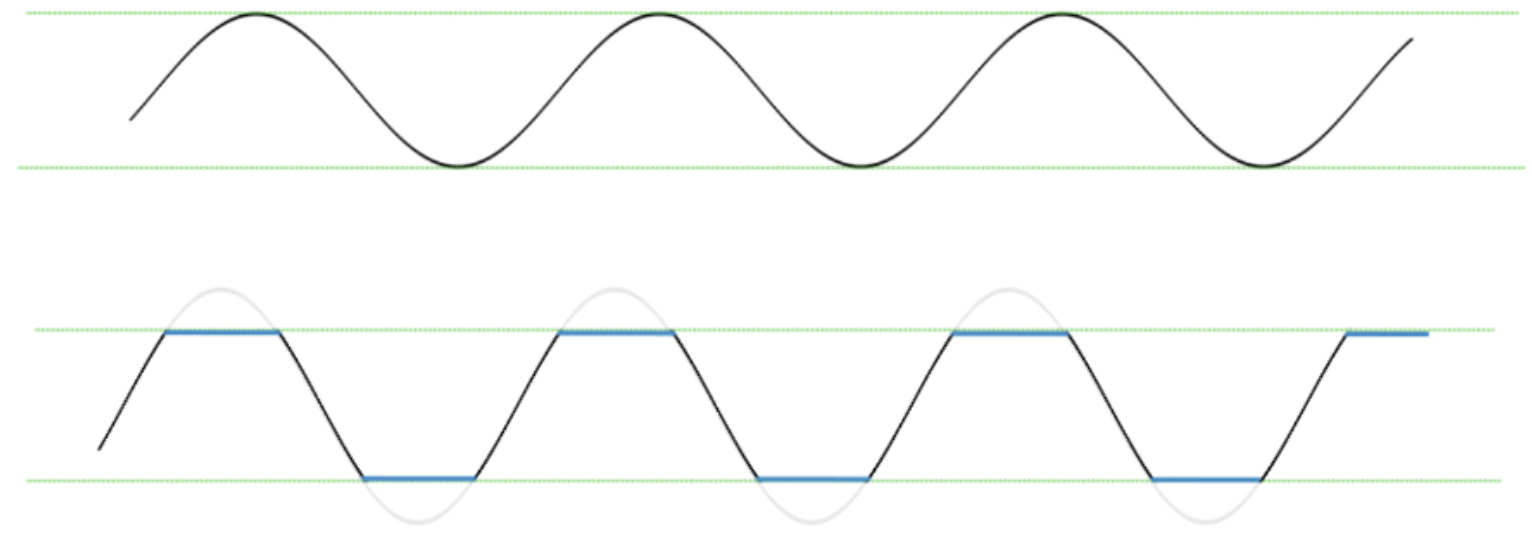
\includegraphics[width=0.7\linewidth]{Clipping}
				\end{center}
			\end{figure}
\newpage
\section{IDEA GENERATION}
\vspace{-5mm}
\rule{\linewidth}{0.1mm}
\normalsize
	\subsection{BRAINSTORMING}
	\subsection{FIRST IDEA}
		This idea was found from the foundation of one of the team member's fascination with space and all things military. The
		idea is that of reducing noise on a signal from space communication. 
		Such signals like satellite communication, military communication, aviation communication and even GPS feedback can all be distorted in Space.
		The distortion occurs when a signal is sent through the atmosphere and things like particles in the air interfere. 
		The team found it interesting how a signal can encounter interference in what seems like open space.
		In reality, there are many things that can affect a signals message in the atmosphere.
		It would have been interesting to see how such a signal could be filtered to reduce noise.\cite{ESA}
	\subsection{SECOND IDEA}
		Another idea that was investigated was using a software defined radio to replicate the signal from a key fob. 
		An SDR is a type of radio communication system that uses software to define and process the transmitted and received signals. 
		The idea was that we could consensually replicate the unique frequency from a team member's car keys in order to unlock the car. 
		A car's key fob contains a small radio transmitter with a unique code. 
		The car receives the signal and decodes it, only if it is deemed correct will the car unlock. 
		If the signal being sent from the key fob transmitter was able to be read in and copied, technically sending that frequency into the car's receiver should unlock the doors.
	\subsection{FINAL IDEA}
		The final idea was a combination of two interests shared among the group members.\\
		Firstly, the sci-fi novel “Project Hail Mary” by Andy Weir. The character Rocky is an alien who speaks in notes and chords. Grace, the main character, uses two laptops, one with an excel spreadsheet for new words, and one running a real time fourier analysis of Rocky’s speech. Everytime a new word is spoken, Grace would check to see which notes make it up. After that, we created a program which looked up the chords on the excel and would translate Rocky’s speech for him. This was such an interesting and new use of the Fourier transform. An application based on this property seemed like a good direction to go down.\\
		Many of the group members share a love of music and play a variety of instruments, but mainly guitar. Inspired by guitar tuners, which show the notes played when a string is plucked, the final project idea was formed.\\
		A software application of the note detecting property of fourier transforms, with a real world application that has actual use. The proposal of the idea to the group was met with an ecstatic reaction and it was settled.\\
	
\newpage

\Large
\section{FINAL IMPLEMENTATION}
\vspace{-5mm}
\rule{\linewidth}{0.1mm}
\large
	\normalsize
	\subsection{OVERVIEW}
			The final project idea is a local web app written in JavaScript that is able to take in live audio input from a guitar, break it into its frequencies and tell the user which chord is being
			played. This concept was expanded upon with a user interface capable of showing the user how the chord would be played on a piano. Most of the code written by the team was written within the 
			Javascript files located in the code base, other files were used to simply get the local app working. The p5.js library was used as it makes visuals more convenient and hosts an FFT 
			object. The project aims to showcase a real world application of convolution, filtering and frequency analysis.
	\subsection{CODE BASE}
			The application is made up of a series of JavaScript files working in tandem to achieve the desired user experience. It implements objected oriented programming techniques. 
			To further illustrate what these files are, as well as show how they interact with each other, the following UML diagram was designed.\\
			\begin{figure}
				\begin{center}
					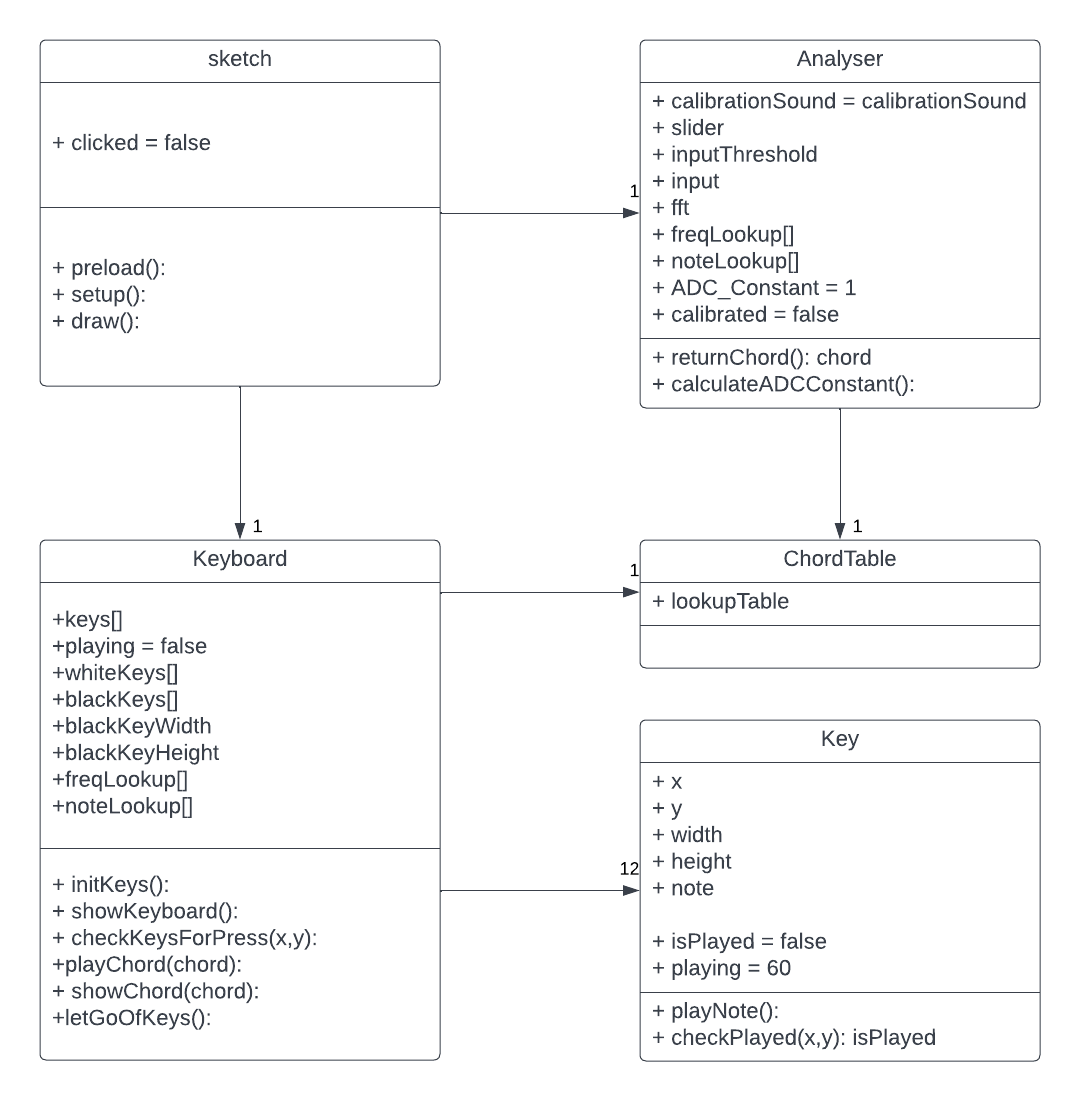
\includegraphics[width=\linewidth]{UML}
				\end{center}
				\caption{UML diagram of code base}
			\end{figure}

\newpage
\vspace*{5mm}

			Below is a detailed explanation of some code snippets of interest within the code base.\\
			\textbf{Sketch.js}\\
			\normalsize
			\begin{lstlisting}
				var keyboard, analyzer, clicked, calibrationSound;
				//preloading sound file for the analyzer calibration sequence
				function preload(){
 					 calibrationSound = loadSound('assets/1-Ab.mp3');
				}
				function setup() {
				     createCanvas(800, 800);
  					 keyboard = new Keyboard();
  					//above sound file is passed in
  					analyzer = new Analyzer(calibrationSound);
  					clicked = false;
				}

			   function draw() {
  			   		//checking to see if a specific key has been pressed
  					if(mouseIsPressed){
    					keyboard.checkKeysForPress(mouseX, mouseY);
  			   		}

      			   var chord = analyzer.returnChord();
  				   if(chord.length > 0) console.log(chord);

		     	   var chord = "A"
				   //shows and plays chord when mouse is clicked
				   var mouseWithinCanvas = (mouseX < width && mouseX > 0 && mouseY < height && mouseY > 0);
				   if(!mouseIsPressed && clicked && mouseWithinCanvas){
					   keyboard.playChord(chord);
					   keyboard.showChord(chord);
				   }

		           background(51);
		           keyboard.showKeyboard();
		           clicked = mouseIsPressed;
		      }
			\end{lstlisting}
			The Sketch.js file contains the main loop of the application. It handles basic setup before the program runs, such as preloading files, setting up the canvas for the UI, etc.
			The draw function is the main loop of the entire codebase, it runs the UI at $60$ frames per second and contains some basic functionality to allow the user to click around on the
			canvas and call certain features.\\
			Within the setup function, two objects are created, the Analyzer and the Keyboard objects. These objects' functions and purposes are detailed below.
\newpage
			\textbf{Analyzer.js}\\
			\normalsize
			The Analyzer object is where the FFT and analysis of the live audio input is performed. It contains two main functions. $returnChord()$ listens to the live audio input, runs an FFT on the 
			signal and fills an array with the frequencies that make it up. $calculateADConstant()$ calibrates the ADC constant for the system and ensures the frequencies are accurate regardless of 
			what kind of hardware it's running on.\\
			\begin{lstlisting}
				calculateADCConstant()
				{
					//known frequency of the sound file
					var testFreq = 415.305;
					var testFFT = new p5.FFT(0.8, 16384);
					testFFT.setInput(this.calibrationSound);
			
					this.calibrationSound.play();
					this.calibrationSound.amp(1);
			
					//the sampling is done after the sound file has been playing for 1500ms
					setTimeout(()=>{
						//stores an array of magnitudes
						var freqSpectrum = testFFT.analyze();
						//used to store frequencies above a certain volume threshold
						var obtainedFreqs = [];
				
						//if a certain frequency is above a certain threshold, it is added
						for(var i = 0; i < freqSpectrum.length; i++)
							if(freqSpectrum[i] > 164) obtainedFreqs.push(i);            
						
						//averaging array
						var avg = 0;
						for(var i = 0; i < obtainedFreqs.length; i++)
							avg += obtainedFreqs[i];
						
						avg /= obtainedFreqs.length;
			
						//setting the ADC_Constant as the ratio between what the reading should be, 
						//and the obtained frequency from the FFT
						this.ADC_Constant = testFreq / avg;
						console.log("ADC_Constant = ", this.ADC_Constant);
						this.calibrated = true;
					}, 1500);
				}
				\end{lstlisting}
					The $calculateADCConstant()$ function ensures the frequency value calculated from the $analyze()$ function is correct and not hardware dependant. The functionality is as follows:
					\begin{itemize}
						\item Lines 4-9\\
							These lines initialise some useful variables and play the calibration sound. 
							$testFreq$ is the known frequency of the calibration sound file. $testFFT$ is the temporary FFT object used to analyse the sound file.
						\item Lines 12-34\\
							This entire block of code is executed after the sound file has been playing for $1500ms$. Once this time has elapsed, the sound file is sampled. Similarly to the $returnChord()$ function,
							only frequencies of a substantial magnitude are let through. Once the array of samples has been filled, an average frequency value is found. The ADC constant is set as the ratio between
							what the analyze function thinks the frequency value is and what it actually is. 
					\end{itemize}
\newpage
			\begin{lstlisting}
	returnChord(){
        var freqSpectrum = this.fft.analyze();
        var noteFrequencies = [];
        var notes = [];

        var baseFrequencies = [131, 139, 147, 156, 82, 87, 92, 98, 104, 110, 117, 123];
        //updating threshold with current value of the on screen slider
        this.inputThreshold = this.slider.value();

        //gathering loudest frequencies from the live input
        for(var i = 0; i < freqSpectrum.length; i++)
        {
            if(freqSpectrum[i] < this.inputThreshold) {continue;} // threshold amplitude
            // var adjustedFreq = round(i * this.ADC_Constant); //frequency value is correct once it is multiplied by the constant 
            var adjustedFreq = i * this.ADC_Constant; //frequency value is correct once it is multiplied by the constant 

            //desired frequency range
            if(adjustedFreq > 75 && adjustedFreq < 550)
                noteFrequencies.push(round(adjustedFreq)); 
        }

        //putting notes into the notes array based on the frequencies found above
        
        for(var p = 0; p < noteFrequencies.length; p++)
        {
            // tuning threshold to be a quarter tone above and below the desired note
            var tuningThreshold = (noteFrequencies[p] * pow(2,(0.042))) - noteFrequencies[p];
            for(var i = 0; i < baseFrequencies.length; i++)
            {
                if((noteFrequencies[p]+tuningThreshold)%baseFrequencies[i] <= tuningThreshold ||
                    (noteFrequencies[p]-tuningThreshold)%baseFrequencies[i] <= tuningThreshold){
                    notes.push(this.noteLookup[i]);
                }
            }
        }

        return notes;
    }
			\end{lstlisting}
		\begin{itemize}
			\item Lines 2-4\\
					These lines declare some variables that are filled as the function progresses. $freqSpectrum$ is filled by the $.analyze()$ function of the FFT object. This array contains $2^{14}$
						values of magnitude ranging from $0-255$. The index of these magnitudes into the array gives its frequency. For example $freqSpectrum[200] == 32$ has a frequency of 200 and a 
						magnitude of 32.
			\item Lines 11-20\\
					These lines dictate which frequencies will be stored in the $noteFrequencies$ array. The algorithm begins by ensuring frequencies with magnitudes below a certain threshold are 
					not included in the final output. This reduces noise and ensures only significant parts of the input signal are taken into account. Once a frequency with a significant magnitude
					is found, it's frequency in Hz is calculated. This calculation is done using the ADC constant.
					The frequency is sent through a bandpass filter to ensure it is within the realistic frequency range of what a guitar can achieve.
					Once a frequency has met all the required criteria, it is pushed to the $noteFrequencies$ array for further analysis.
			\item Lines 24-35\\
					These lines of code attempt to detect which note is being played, regardless of octave. This technique uses thresholding and some of the relationships between frequency and musical
					note detailed in Section 5.2: Music Theory.\\
					The algorithm makes use of the fact that for any given frequency the next musical half tone follows the following formula:
					$$
						nextFrequency = baseFrequency * 2^{\frac{1}{12}}
					$$
					This section is similar to a bandpass filter where a range of frequencies is let through. Since it is unlikely that the input frequency will be the exact frequency
					desired for a particular note. If the frequency being tested is within a certain tuning threshold, it is set to be the note that it is close to. \\
					The $tuningThreshold$ variable stores the acceptable difference in frequency. Since the difference between a note's frequency and the frequency of the note a half-tone
					above scales with frequency, this value must be calculated for each value.\\
						For example, the difference between an $A_2$ $(110Hz)$ and an $A\#_2$ is as follows:
						$$
							(110 * 2^{\frac{1}{12}}) - 110 = 6.54Hz
						$$
						While the difference between an $A_{4}$ $(440Hz)$ and an $A\#_4$ is given as:
						$$
							(440 * 2^{\frac{1}{12}}) - 440 = 26.163Hz
						$$
\newpage
\vspace*{5mm}
					The threshold is set to be the frequency being tested $\pm$ a quarter tone from that frequency. The statement at line 30 tests the difference between the upper
					bound and the note frequency and the lower bound and the note frequency. The modulo operator is used to test for this threshold regardless of harmonic.
						For example if an $A_4$ $(440Hz)$and $A_3$ $(220Hz)$were being tested against an $A_2$ $(110Hz)$. The threshold would be calculated as $$440hz \% 110Hz = 0$$
						\begin{center}and\end{center} $$220Hz \% 110Hz = 0$$
						Once a note has satisfied being within the frequency range of a particular note, that note is added to the $notes$ array.
					\normalsize
		\end{itemize}

\newpage

\vspace*{5mm}
		The calculateADCConstant() function was deemed necessary as the application gave different frequency values on different teams members' laptops. Initially, it was assumed that the difference was due to the
		microphones sampling rates. An external microphone was used to test this theory. The frequencies stayed the same no matter what microphone was used, signifying that it was an issue with 
		how the laptops handled sound internally.
		The calibration solution works perfectly and calculates each laptops unique constant consistantly.

		The application has some visual aspects to it that allow the user to see which chord is being played. The app can play a given musical chord audibly, as well as visually. A lookup table
		of chords was created that allows the program to know which notes to play to make up that chord. A snippet of the chord table is shown below.\\
		\begin{lstlisting}
class chordTable{
    constructor(){
        //lookup table for chords
        //first column contains chord names 
        //while the rest of the row contains the notes needed to make up that chord
        this.lookupTable = [
            //major
            ["C", "C", "E", "G"],
            ["C#", "C#", "F", "G#"],
            ["D", "D", "F#", "A"],
            ["D#", "D#", "G", "A#"],
            ["E", "E", "G#", "B"],
            ["F", "F", "A", "C"],
            ["F#", "F#", "A#", "C#"],
            ["G", "G", "B", "D"],
            ["G#", "G#", "C", "D#"],        
            ["A", "A", "C#", "E"],
            ["A#", "A#", "D", "F"],
            ["B", "B", "D#", "F#"],
            //minor
            ["Cm", "C", "D#", "G"],
            ["C#m", "C#", "E", "G#"],
            ["Dm", "D", "F", "A"],
            ["D#m", "D#", "F#", "A#"],
            ["Em", "E", "G", "B"],
            ["Fm", "F", "G#", "C"],
            ["F#m", "F#", "A", "C#"],
            ["Gm", "G", "A#", "D"],
            ["G#m", "G#", "B", "D#"],        
            ["Am", "A", "C", "E"],
            ["A#m", "A#", "C#", "F"],
            ["Bm", "B", "D", "F#"]
	}
}		
		\end{lstlisting}

		The above is a shortened version of the chord lookup table. It has been shortened for brevity. The chord table in the code base contains augmented, diminished, major and minor 7ths, and suspended
		2nd and 4th chords. The code shown below showcases how this table can be used to synthesise chords and play them to the speakers.
\newpage
	
		\textbf{Keyboard.js}\\
		\normalsize
	\begin{lstlisting}
	//sets up oscillator objects and synthesises frequencies into a single one
    playChord(chord){

        var audio = new AudioContext();
        //stores oscillator objects for each of the required frequencies
        var oscillators = [];
        //gain is used to reduce clipping of the final signal
        var sigGain = audio.createGain();
        //searching for chord elements in lookup
        var posInLookup = 0;

        for(var i = 0; i < this.chordLookup.length; i++){
            if(this.chordLookup[i][0] == chord){
                posInLookup = i;
                break;
            }
        }
        //scales gain of each note based on number of notes in a chord
        sigGain.gain.value = 1 / (this.chordLookup[posInLookup].length - 1);

        //creating new oscillators, adding them to the array and setting their frequencies
        for(var i = 1; i < this.chordLookup[posInLookup].length; i++){
            var tempOscillator = audio.createOscillator();
            oscillators.push(tempOscillator);

            var freqOfNote = 0;

            for(var j = 0; j < this.noteLookup.length; j++){
                if(this.chordLookup[posInLookup][i] == this.noteLookup[j]){
                    freqOfNote = this.freqLookup[j]; //getting the frequency of each note
                }
            }
            oscillators[i - 1].frequency.value = freqOfNote; //setting an oscillators frequency
            oscillators[i - 1].connect(sigGain); //attaching the oscillator to the Gain node
        }
        sigGain.connect(audio.destination);

        //starting oscillators
        for(var i = 0; i < oscillators.length; i++)
            oscillators[i].start(0);
        
        //adds fade out
        setTimeout(()=>{
            sigGain.gain.exponentialRampToValueAtTime(0.0000001, audio.currentTime + 10)
        }, 1000);
    }
\end{lstlisting}

	The $playChord()$ function shown above is capable of taking in a chord as a string, determining which notes make up that chord, and playing the chord to the speakers after synthesising together
	the required frequencies. 
	\begin{itemize}
		\item Lines 4-17\\
				Initialises required variables used in that function. The loop finds the correct position in the chord lookup table so that the required notes can be found. 
\newpage
\vspace*{5mm}
		\item Line 19\\
				The $sigGain$ variable is an audio gain node. Each of the sine wave oscillators will be attached to this gain node. The gain value is set to be $\frac{1}{numOfNotes}$. 
				This is done to remove possible clipping of the signal, and keep amplitude between chords of differing length consistent. 
		\item Lines 22-36\\
				This section creates sine wave oscillators and connects them to the gain node mentioned above. It does this by first finding the correct frequency for each note. Within the keyboard
				object, a member variable, $freqLookup$ exists which contains the frequencies of each note at a set octave. Once the oscillators have been created, it is connected to the gain node at
				line 34.
	\end{itemize}
	From here, the oscillators are started and the synthesised signal is played to the speaker. The $setTimeout()$ function on line 43 is used to gradually reduce the chord's amplitude until it is not
	playing. This reduces the 'pop' that can occur at the end of audio signals where the signal is stopped when it is a non-zero value.
\begin{figure}[h]
	\begin{center}
		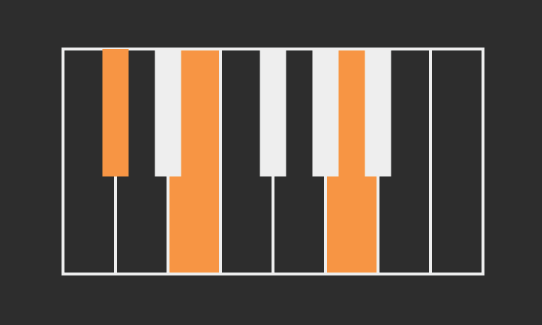
\includegraphics[width=0.7\linewidth]{Piano}
	\end{center}
	\caption{UI playing an A major}
\end{figure}
	Above is an example of the UI playing an A major chord.
\newpage
\vspace*{5mm}
		While the thresholding algorithm still requires more testing, the application's ability to break a chord
		into its frequencies is consistent. Figures 15 and 16 show the application successfully 
		picking up the frequencies that make up an $A$ and $A_{7}$ chord respectively.\\
		\begin{figure}[H]
			\begin{center}
					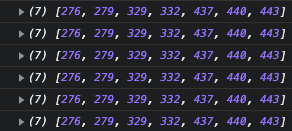
\includegraphics[width=0.7\linewidth]{A_Chord_Javascript}					
			\end{center}
			\caption{Javascript Application successfully breaking down an $A$ chord into its frequencies}
			\label{fig:A_Chord_Javascript}
		\end{figure}
		Figure \ref{fig:A_Chord_Javascript} shows the output of the application when an $A$ chord was played into the live audio 
		input of the application. Each of the frequencies above lie close to the core frequencies of an $A$ at this
		octave. $A$ $(440Hz)$, $C\#$ $(277Hz)$ and $E$ $(329Hz)$. 
		\begin{figure}[H]
			\begin{center}
				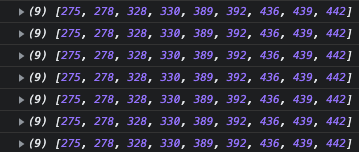
\includegraphics[width=0.7\linewidth]{A7_Chord_Javascript}
			\end{center}
			\caption{Javascript Application successfully breaking down an $A_{7}$ chord into its frequencies}
			\label{fig:A7_Chord_Javascript}
		\end{figure}
		Figure \ref{fig:A7_Chord_Javascript} shows the output of the application when an $A_{7}$ was played. This test was performed
		as a $7^{th}$ chord is a four note chord. The frequencies output will be a regular triad with an added
		note. This added note, $G$ $(392Hz)$ can be seen in the output of the application, alongside the notes
		that make up the base $A$ triad.
\newpage
	\subsection{IMPLEMENTATION IN MATLAB}
		Matlab is used to show the direct application of the underlying theory\cite{CodeTutorial}. This section examines the code and shows how this theory applies to the solution.\\
		Taking in the audio file\cite{AudioFiles}:
			\begin{lstlisting}
				[y,fs] = audioread('2-Ab-C-Dyad.mp3');
				info = audioinfo('2-Ab-C-Dyad.mp3')
			\end{lstlisting}
		$audioread()$ takes in a file containing audio data (.mp3, .mp4, .wav), and automatically samples it.\\
		$'y'$ is the audio data, and is returned as an $m$ x $n$ matrix.
		\begin{itemize}
			\item[] m = No. of samples
			\item[] n = No. of audio channels
		\end{itemize}
		The audio files included within the project have stereo channels $(n = 2)$.\\
		$'fs'$ is the audio sampling rate, in $Hz$.\\
		$'audioinfo()'$ returns data about the audio file.

		\begin{figure}[H]
			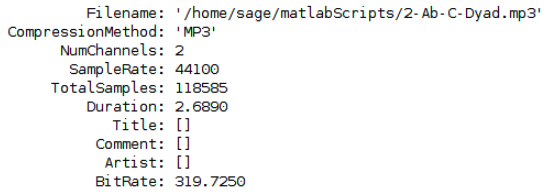
\includegraphics[width=0.7\linewidth]{audioinfo}
			\caption{Information returned from $audioinfo()$ function}
		\end{figure}
		Resampling\cite{Resample}:\\
		\begin{lstlisting}
			y = y(:,1); %reducing to one channel
			y_res = resample(y,20000,fs) %resample to reduce data size
		\end{lstlisting}
		The first column of the sampled signal is taken to reduce the size of the data. This will help
		with processing speed.\\
		$'resample()'$: y is resampled at a rate of $20000/fs$ times y's sample rate. Since this is 
		already $fs$, the result $y_{res}$ will have a sampling rate of $20kHz$.\\
		The function resamples y with a finite impulse response antialiasing lowpass filter.\\
		The new sampling rate $20kHz$ os the Nyquist frequency of $fs$. Using this and the filter from
		$resample()$, the aliasing is further decreased. $y_{res}$ will be used to create a spectograph.\\
		\emph{Note:} the maximum musical note frequency applicable is $7902.13Hz$ ($A^b_8$)\cite{NoteReference}. To ensure
		the frequencies of interest don't alias, and because lowpass filters cannot have an infinitely steep
		cutoff slope, the sampling rate must be at least twice this. This is another reason why $20kHz$ is
		used. \vspace*{5mm} It's Nyquist frequency is $10kHz$, well above the max input frequency of interest.\\

		Time domain plot of audio file:
		\begin{lstlisting}
%time domain
%t = 0 to y/fs, spaced evenly via y steps
t = linspace(0,length(y)/fs,length(y));
figure
plot(t,y);
title('Time Domain');
xlabel('time');
ylabel('amplitude');
		\end{lstlisting}
		\begin{figure}[h]
			\begin{center}
			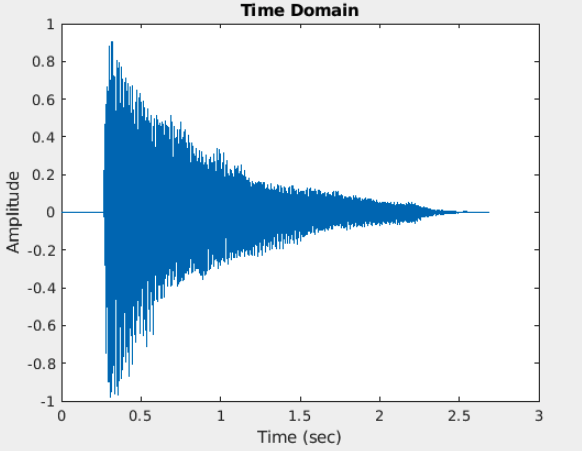
\includegraphics[width=0.7\linewidth]{time_domain_plot}
			\end{center}
			\caption{Time domain plot of audio file}
		\end{figure}
\newpage	
Frequency domain:
		\begin{lstlisting}
y_fft = fft(y); %dft
n = length(y);
f = (0:n-1)*(fs/n); % freq range
power = abs(y_fft).^2/n; %power of dft
[pks,locs] = findpeaks(power, f, MinPeakHeight=16.35);
		\end{lstlisting}
\begin{itemize}
	\item $fft(y)$ performs a fast fourier transform on $y$, as discussed previously.
	\item $n$: stores rhe number of samples.
	\item $f$: an array of frequency the range, to be used on frequency domain graph.
	\item $fs/n$ is the sampling interval.\cite{SamplingInterval}
	\item $power$: computes and stores the power of each frequency component for each sample.
			\begin{itemize}
					\item [] $Power$ = magnitude of the frequency squared = $F(n)\cdot F(n)^{\*} = |F(n)|^{2}$\cite{PowerSpectrum}
					\item [] $/n$ = per sample
			\end{itemize}
	\item $findpeaks()$
			\begin{itemize}
				\item[] $pks$ - local peak values that occured above $10dB/Hz$
				\item[] $locs$ - frequencies at which those peaks occured.
			\end{itemize}
\end{itemize}
Frequency domain plot:
	\begin{lstlisting}
plot(f,power);
hold on;
peaks = plot(locs, pks, 'hexagram', 'MarkerSize',10, 'Color','r');
legend('Individual Notes', 'Peaks');
for i = 1:length(pks)
        datatip(peaks,locs(i), pks(i))
end
	\end{lstlisting}
\newpage
\begin{figure}[h]
	\begin{center}
		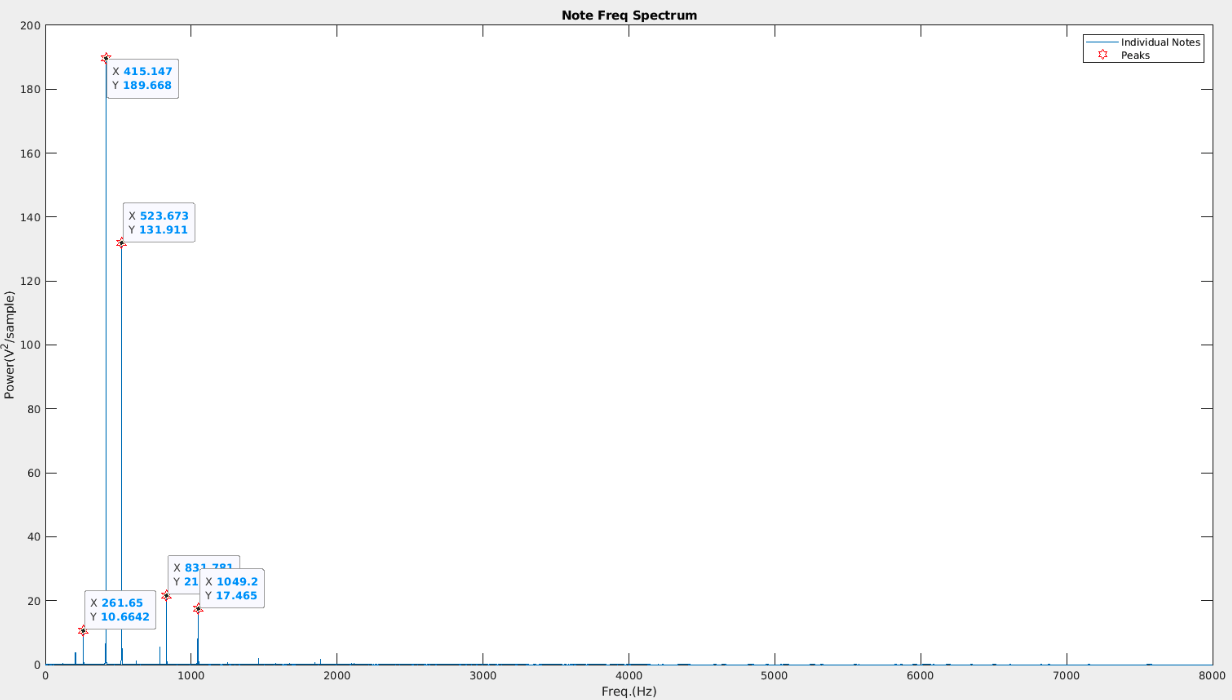
\includegraphics[width=\linewidth]{frequency_domain_plot}
	\end{center}
	\caption{Frequency domain plot of audio file}
\end{figure}
Notes plotted:\\
\begin{center}
	\begin{tabular}{|c|c|}
		\hline
		Frequency(lowest to highest) & Note\\
		\hline
		$261.65$ & $C_4$\\
		$415.147$ & $A^b_{\ 4}$\\
		$523.673$ & $C_5$\\
		$831.781$ & $A^{b}_{\ 5}$\\
		$1049.2$ & $C_6$\\
		\hline
	\end{tabular}
\end{center}
The $.mp3$ file contains an $A^b$ dyad, the fft has successfully broken up the chord into its component
notes.\\
\newpage
\textbf{Spectograph}\\
A spectrograph plots a signal in time, power, and frequency.\\
\begin{figure}[H]
	\begin{center}
		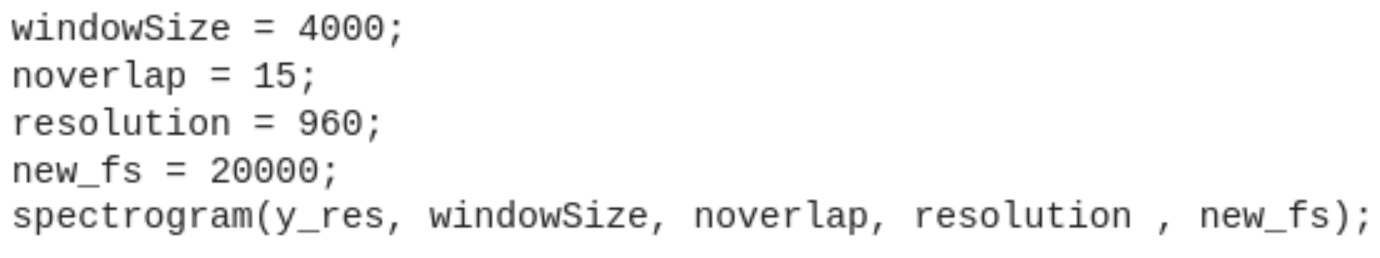
\includegraphics[width=0.7\linewidth]{Spectograph_text}
	\end{center}
	\caption{Spectograph Parameters}
\end{figure}
	\begin{itemize}
		\item $y_{res}$ is the resampled signal.
		\item $windowSize$ 
	\end{itemize}
	\begin{figure}[H]
		\begin{center}
			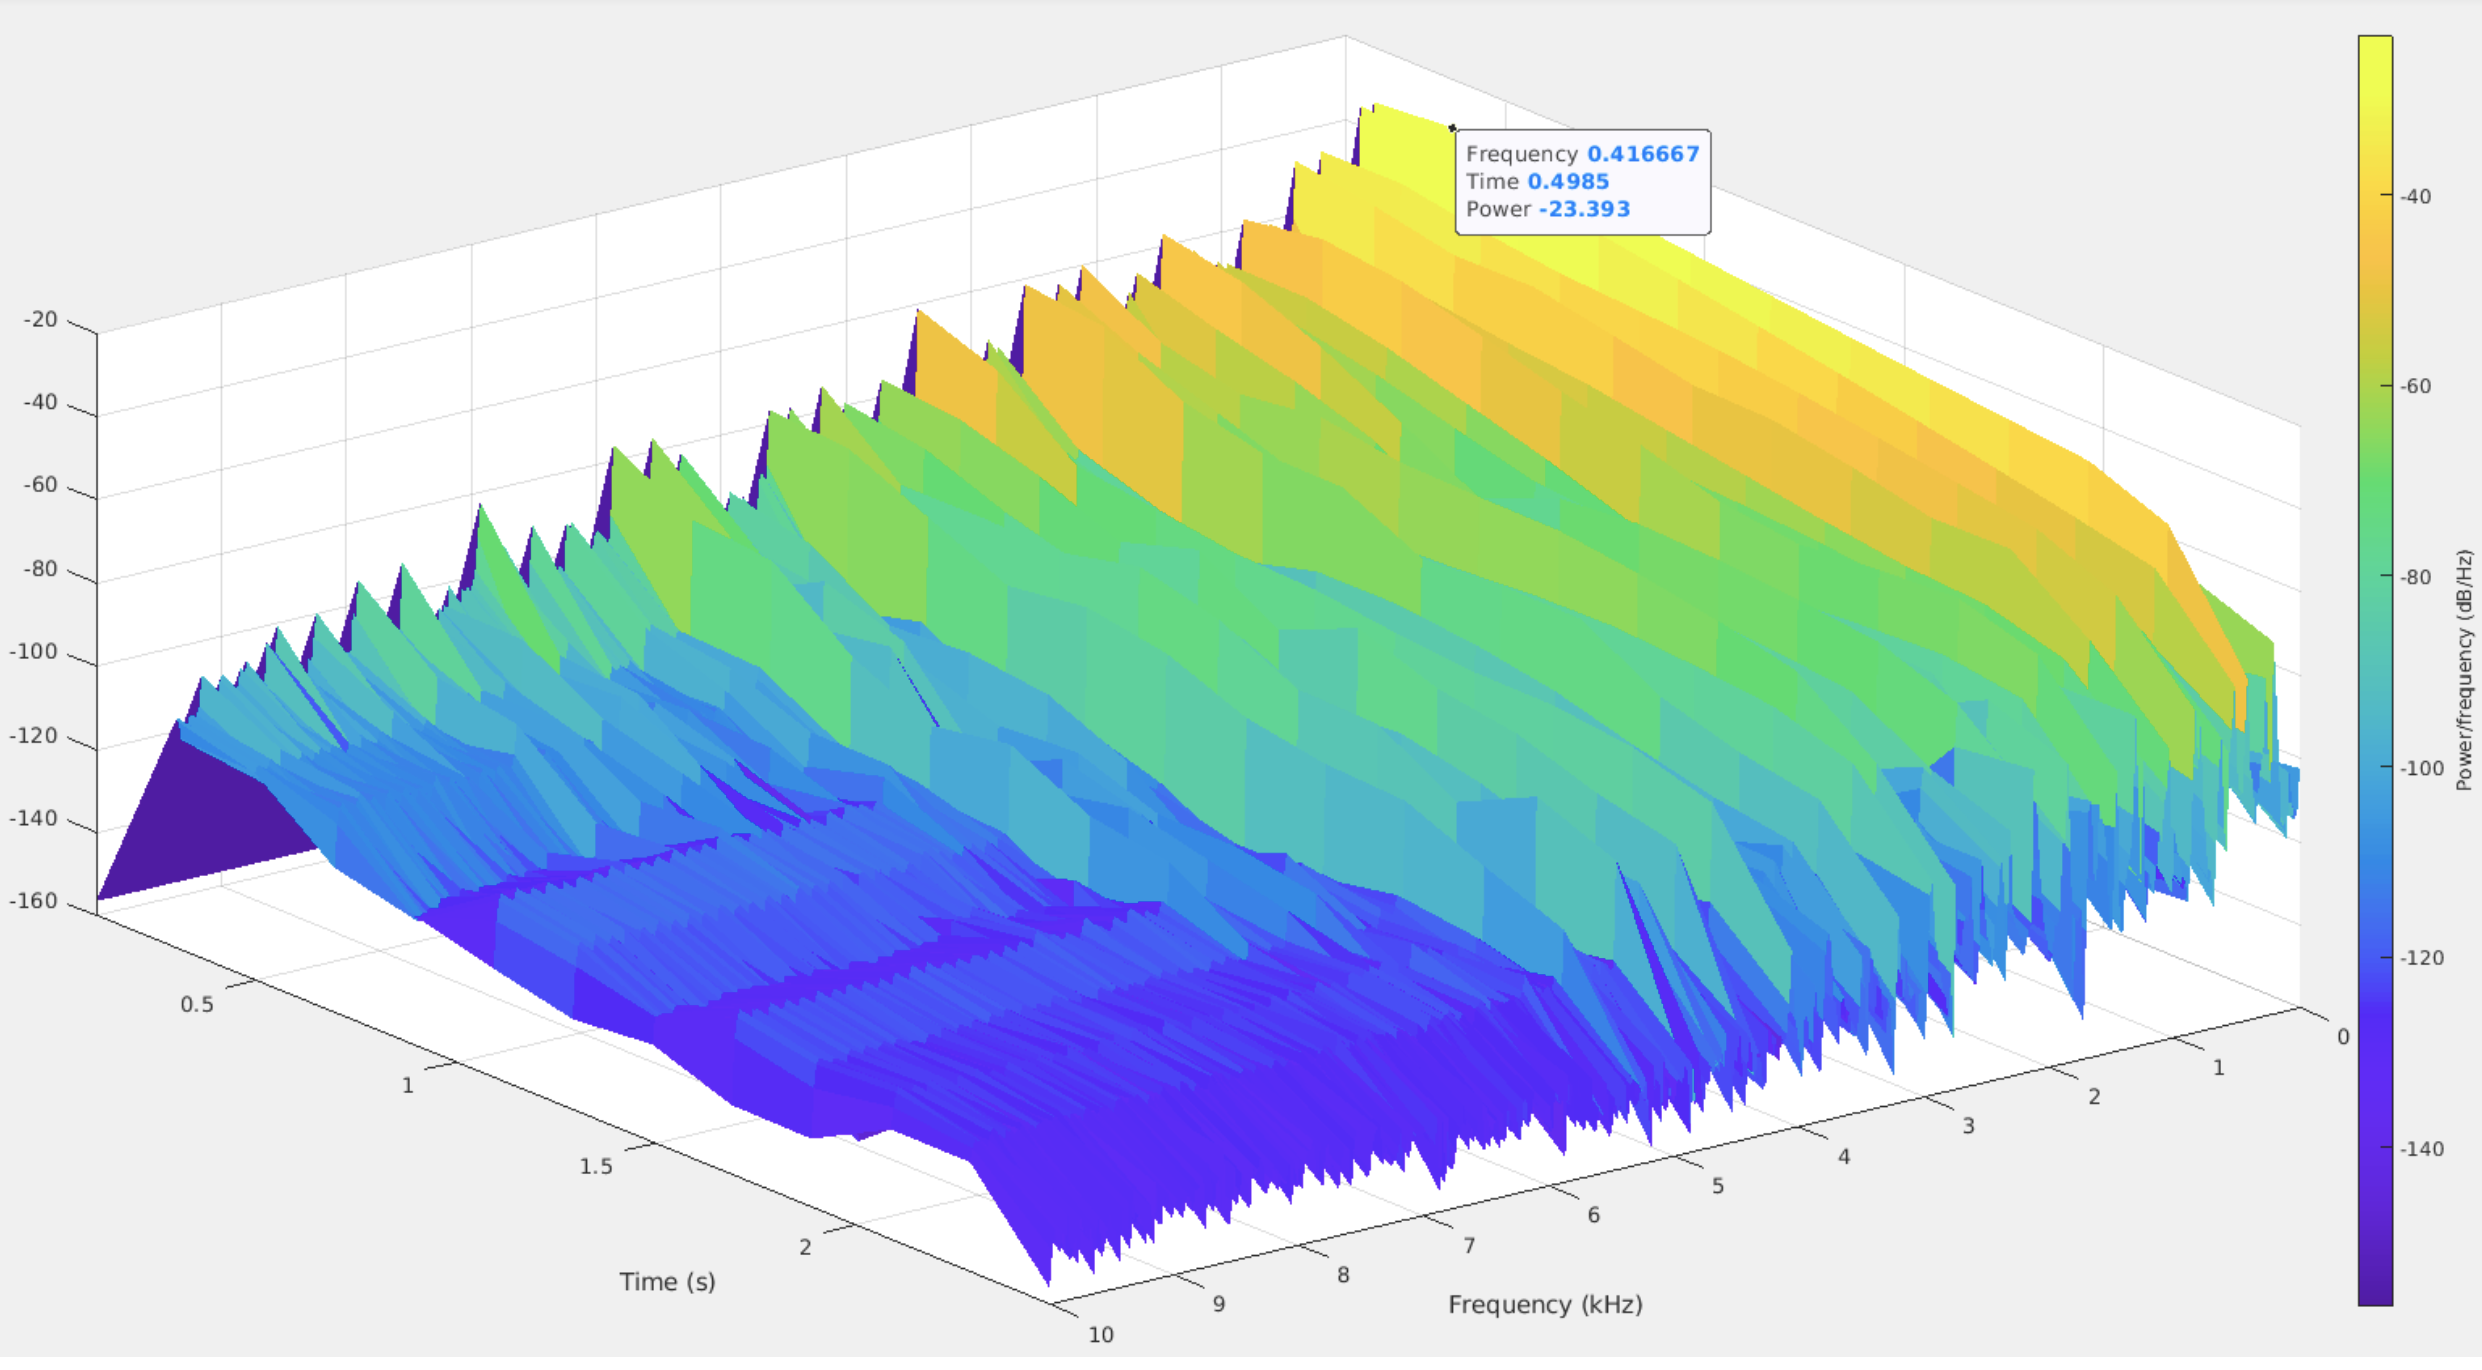
\includegraphics[width=0.9\linewidth]{Spectograph}
		\end{center}
	\end{figure}
\newpage
	\textbf{Aliasing}\\
	In general, aliasing occurs when the sample rate is not fast enough to porberly monitor the system. What we are left with is an error signal from which we cannot reconstruct the original signal.\\
	\begin{figure}[H]
		\begin{center}
			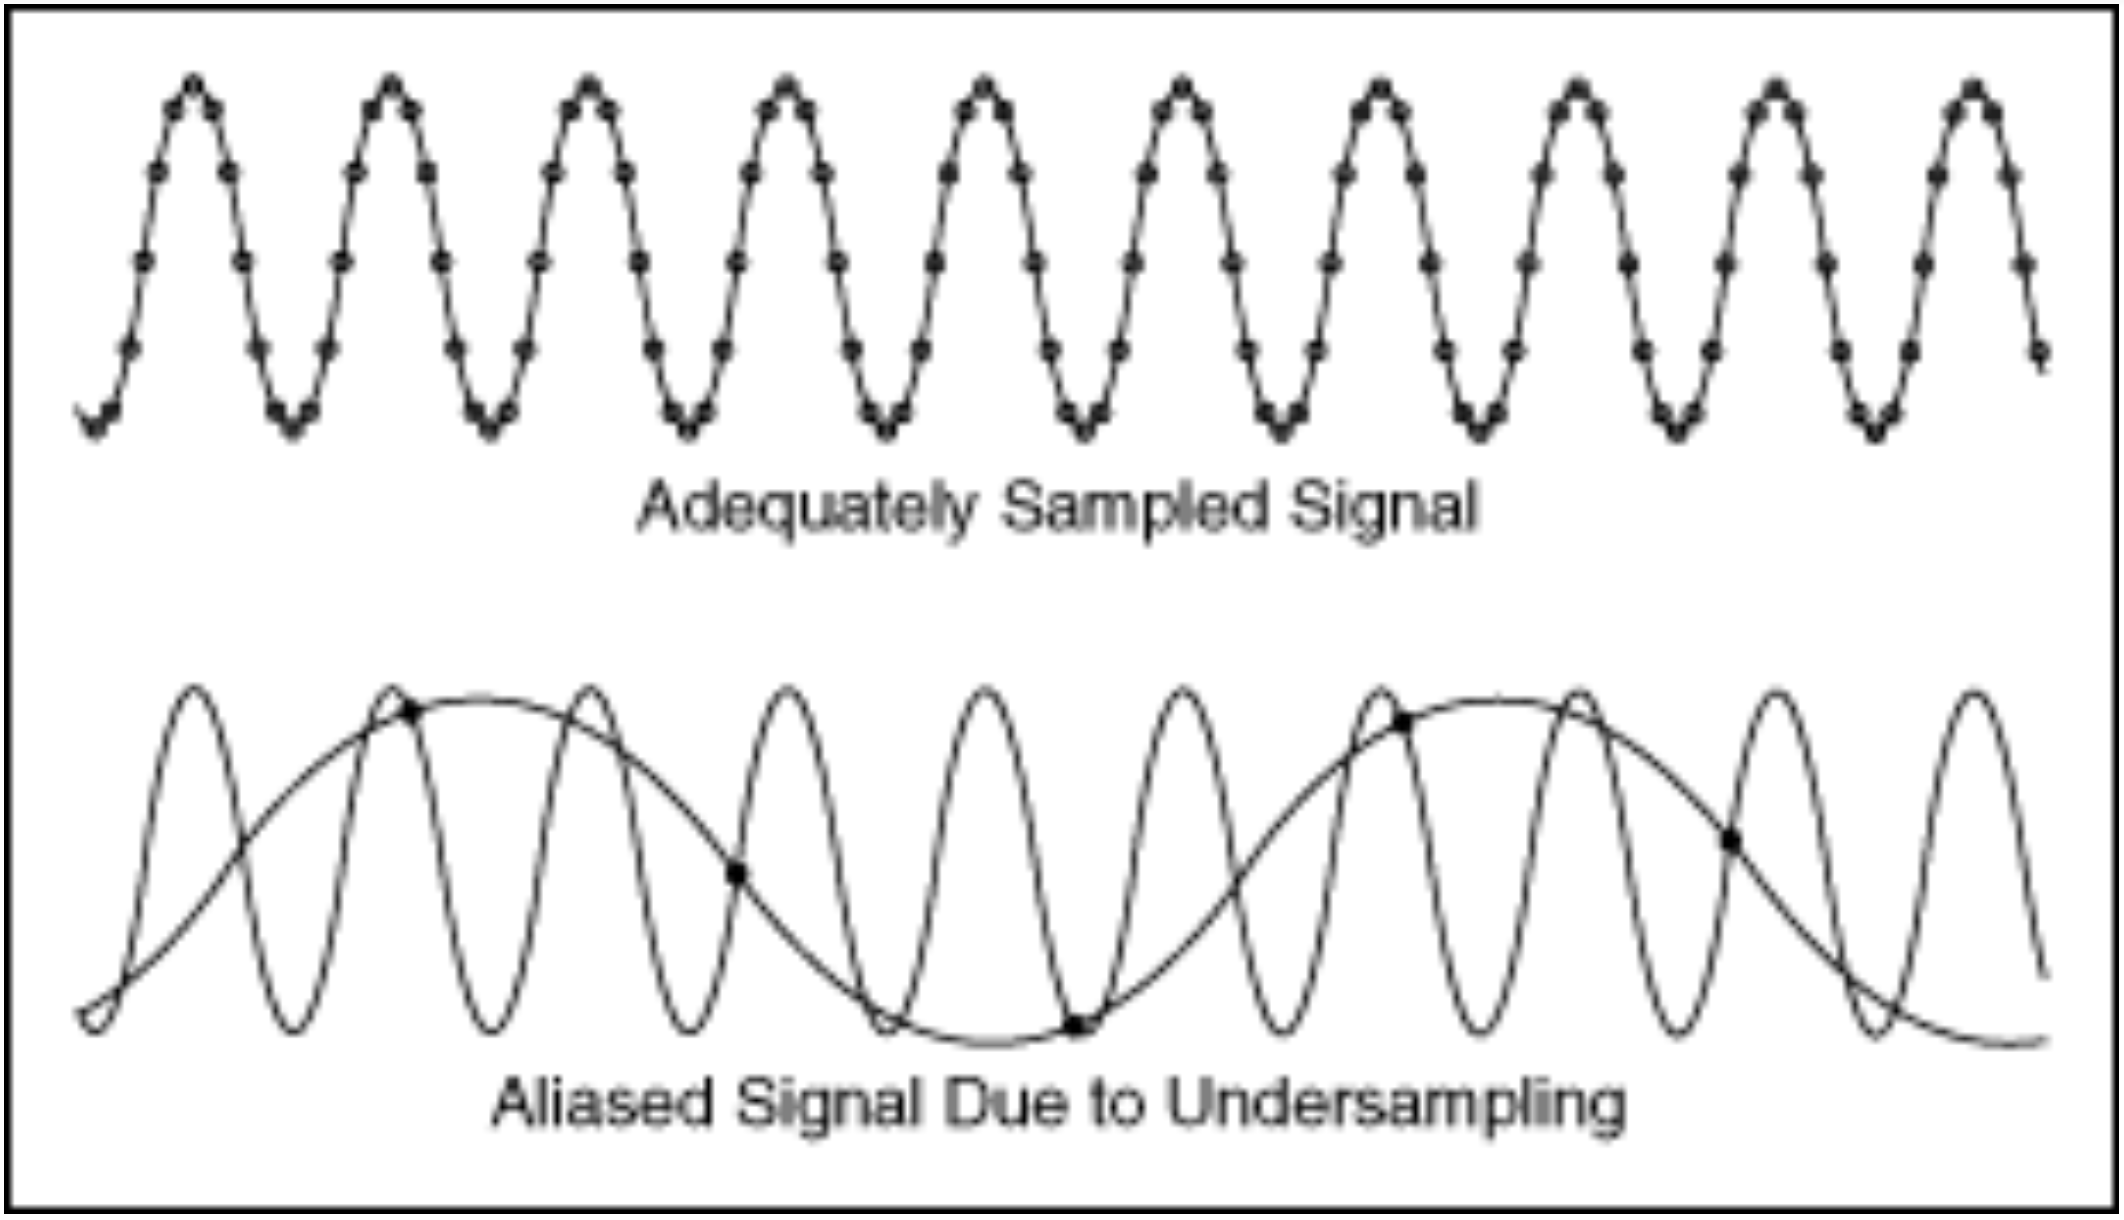
\includegraphics[width=0.7\linewidth]{Aliasing}
		\end{center}
		\caption{Example of Aliasing in a Signal}
	\end{figure}
	As the signal is passed through, the sampling device can’t sample at a regular rate, completely missing the characteristic parts of the wave, meaning it can’t plot the peaks, troughs, amplitude and wavelength.
The resulting signal is completely different from the original, and will form an alias below the nyquist frequency.
Aliases distort the original signal, which is undesirable when the purpose of the project is signal analysis. Often the solution is an anti-aliasing filter.
\\\textbf{Anti-Aliasing Filter}\\
This filter assures any input signal greater than $fs$ is attenuated down as to not form an alias signal that would significantly distort the frequency of interest.
The filter is broken into three parts: Passband, transition region and Stopband
\begin{figure}[H]
	\begin{center}
		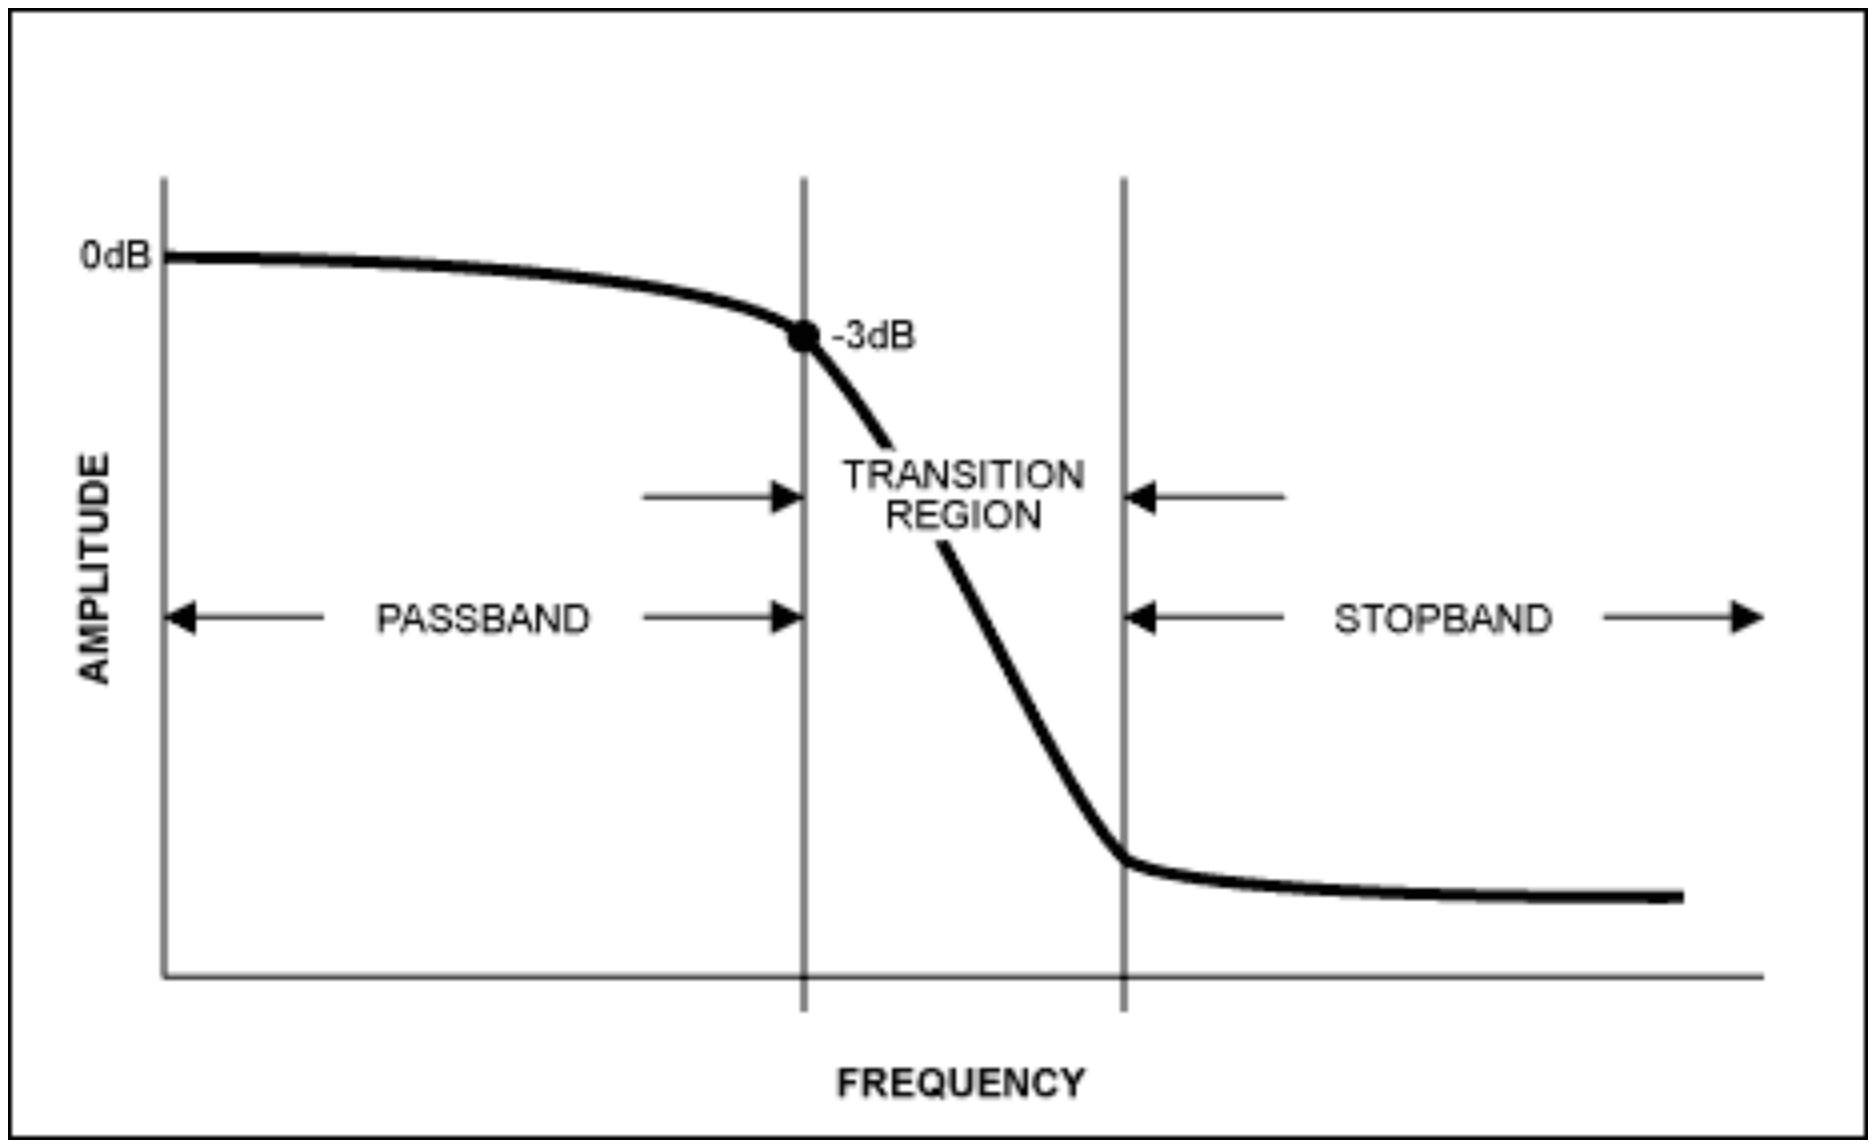
\includegraphics[width=0.7\linewidth]{Aliasing_Filter}
	\end{center}
\end{figure}
This is the same structure as a lowpass filter, with a particular focus on aliases
Frequencies in the passband are left alone, while frequencies in the stop band are significantly attenuated.
It is impossible to get a transition region that is a brick wall shape without infinite hardware, but there is leeway. So long as the end of the region is before the Nyquist frequency, it will work.
Signals above the Nyquist will still form an alias, but these will be attenuated enough to be below the point of distribution.

\newpage
\subsection{POSSIBLE FURTHER WORK}
While the JavaScript application can successfully determine frequencies, the full functionality is not yet
complete. Future work would include doing the inverse of what the $playChord()$ does, where given 
a series of notes, the algorithm can tell the user which chords are being played. The application also
struggled slightly with detecting more than three notes. This means that any chord that is identified
using more than three notes, $7^{th}$ chords, augmented chords, etc. would be inconsistently identified.\\
There is a lot of overlap between notes and different chords, as such, the algorithm can always be improved.
The team would also like to implement a UI element capable of displaying the chord live, above the keyboard.
This could have real world use for musicians.

\newpage
\section{CONCLUSIONS}
\vspace{-5mm}
\rule{\linewidth}{0.1mm}
In conclusion, the team is very happy with how the project turned out.
Despite the fact that the application's full functionality is not yet complete, the team
is confident that, given more time, the app could reach this point. 
The application proved the real world use cases for frequency analysis, 
filtering and convolution - both in frequency and time domains.\\
The theory behind frequency analysis for musical note and chord detection was further
investigated using Matlab.\\
The team also learned a lot about different types of filters. After much research into filters,
their use cases, their advantages and disadvantages, the bandpass and comb filters were deemed
appropriate for this specific use case.

\newpage

\small
\section{BIBLIOGRAPHY}
\vspace{-5mm}
\rule{\linewidth}{0.1mm}
\vspace*{-10mm}
\bibliography{references}
\newpage

\Large
\section{APPENDIX}
\vspace{-5mm}
\rule{\linewidth}{0.1mm}
\large
\textbf{PBL RISK ASSESSMENT FORM}
\normalsize
\begin{center}
		\begin{tabular}{ll}

	\hline
		\multicolumn{1}{|l|}{NAME AND STUDENT NUMBER} &\multicolumn{1}{|l|}{PROJECT NAME:}\\
		\multicolumn{1}{|l|}{Stephen Gallagher - 20470574} & \multicolumn{1}{|l|}{EE301 Project}\\
		\multicolumn{1}{|l|}{Conal Hughes - 20365616} & \multicolumn{1}{|l|}{Musical Chord Detection using Frequency Analysis}\\
		\multicolumn{1}{|l|}{Gerard McIntyre - 20332566} & \multicolumn{1}{|l|}{}\\
		\multicolumn{1}{|l|}{Amy O'Mara - 20386631} &  \multicolumn{1}{|l|}{}\\
		\multicolumn{1}{|l|}{Sage Redmond - 20327943} &  \multicolumn{1}{|l|}{}\\
		\multicolumn{1}{|l|}{Connall Sharkey - 20389076}&  \multicolumn{1}{|l|}{}\\
	\hline
		\multicolumn{1}{|l|}{SUPERVISOR: Dr. Bob Lawlor} & \multicolumn{1}{|l|}{PROJECT LOCATION}\\
		\multicolumn{1}{|l|}{}& \multicolumn{1}{|l|}{EE1.01}\\
	\hline
		\multicolumn{2}{|l|}{BRIEF DESCRIPTION OF PROJECT}\\
		\multicolumn{2}{|l|}{
							 \begin{tabular}{p{0.8\linewidth}}
								 This project’s aim is to take in an input sound from a musical instrument into a microphone and find what chord this sound is. It does so by breaking down the input sound into notes and using a chord look-up table to match what chord suits the sound best. Within our code there are many different functions that reduce the noise on this sound to make it cleaner and easier to identify after being received on the microphone.
							 \end{tabular}
							 } \\
	\hline
	
\end{tabular}
		\vspace{2cm}\\
\begin{tabular}{lll}
		\hline 
			\multicolumn{3}{|l|}{\textbf{Hazards, Risk[High(H), Medium(M) Low(L)], and control measures}}\\\hline
			\multicolumn{1}{|l|}{HAZARD} & \multicolumn{1}{|l|}{Risk} & \multicolumn{1}{|l|}{Controls}\\
			\multicolumn{1}{|l|}{Eye Strain} & \multicolumn{1}{|l|}{M} & \multicolumn{1}{|l|}{Reduce time spent in front of screens and take regular breaks}\\
			\multicolumn{1}{|l|}{Inadequate breaks} & \multicolumn{1}{|l|}{L} & \multicolumn{1}{|l|}{Take breaks when needed.}\\
			\multicolumn{1}{|l|}{Hearing damage} & \multicolumn{1}{|l|}{M} & \multicolumn{1}{|l|}{Always checking volume before playing any kind of signal}\\
			\multicolumn{1}{|l|}{Damage to equipment} & \multicolumn{1}{|l|}{M} & \multicolumn{1}{|l|}{Ensuring level of output signals is at a safe level}\\
			\hline
			\multicolumn{3}{|l|}{
									\begin{tabular}{p{0.9\linewidth}}
										Identified risks should be discussed with your supervisor and a safe system of work agreed. A more in depth risk assessment may be required after initial review. Do not proceed until the form is signed off.
									\end{tabular}
								}\\\hline
\end{tabular}
\end{center}
\newpage

\end{document}
